% ==============================================================================
% 01_similitudes_aerien.tex - Module 1 (08h30 - 10h00)
% Présentation d'un drone sous-marin : similitudes avec le drone aérien
% Conception concrète : BlueROV2, BlueBoat, actionneurs T200, Bar30/Bar02, Navigator
% ==============================================================================

\section{Module 1 : Similitudes avec l'Aérien \& Conception Concrète}

\begin{frame}{1.1 Typologie des 5 Grands Vecteurs Aquatiques Scientifiques}
  \begin{columns}[T]
    \begin{column}{0.19\textwidth}
      \begin{center}
        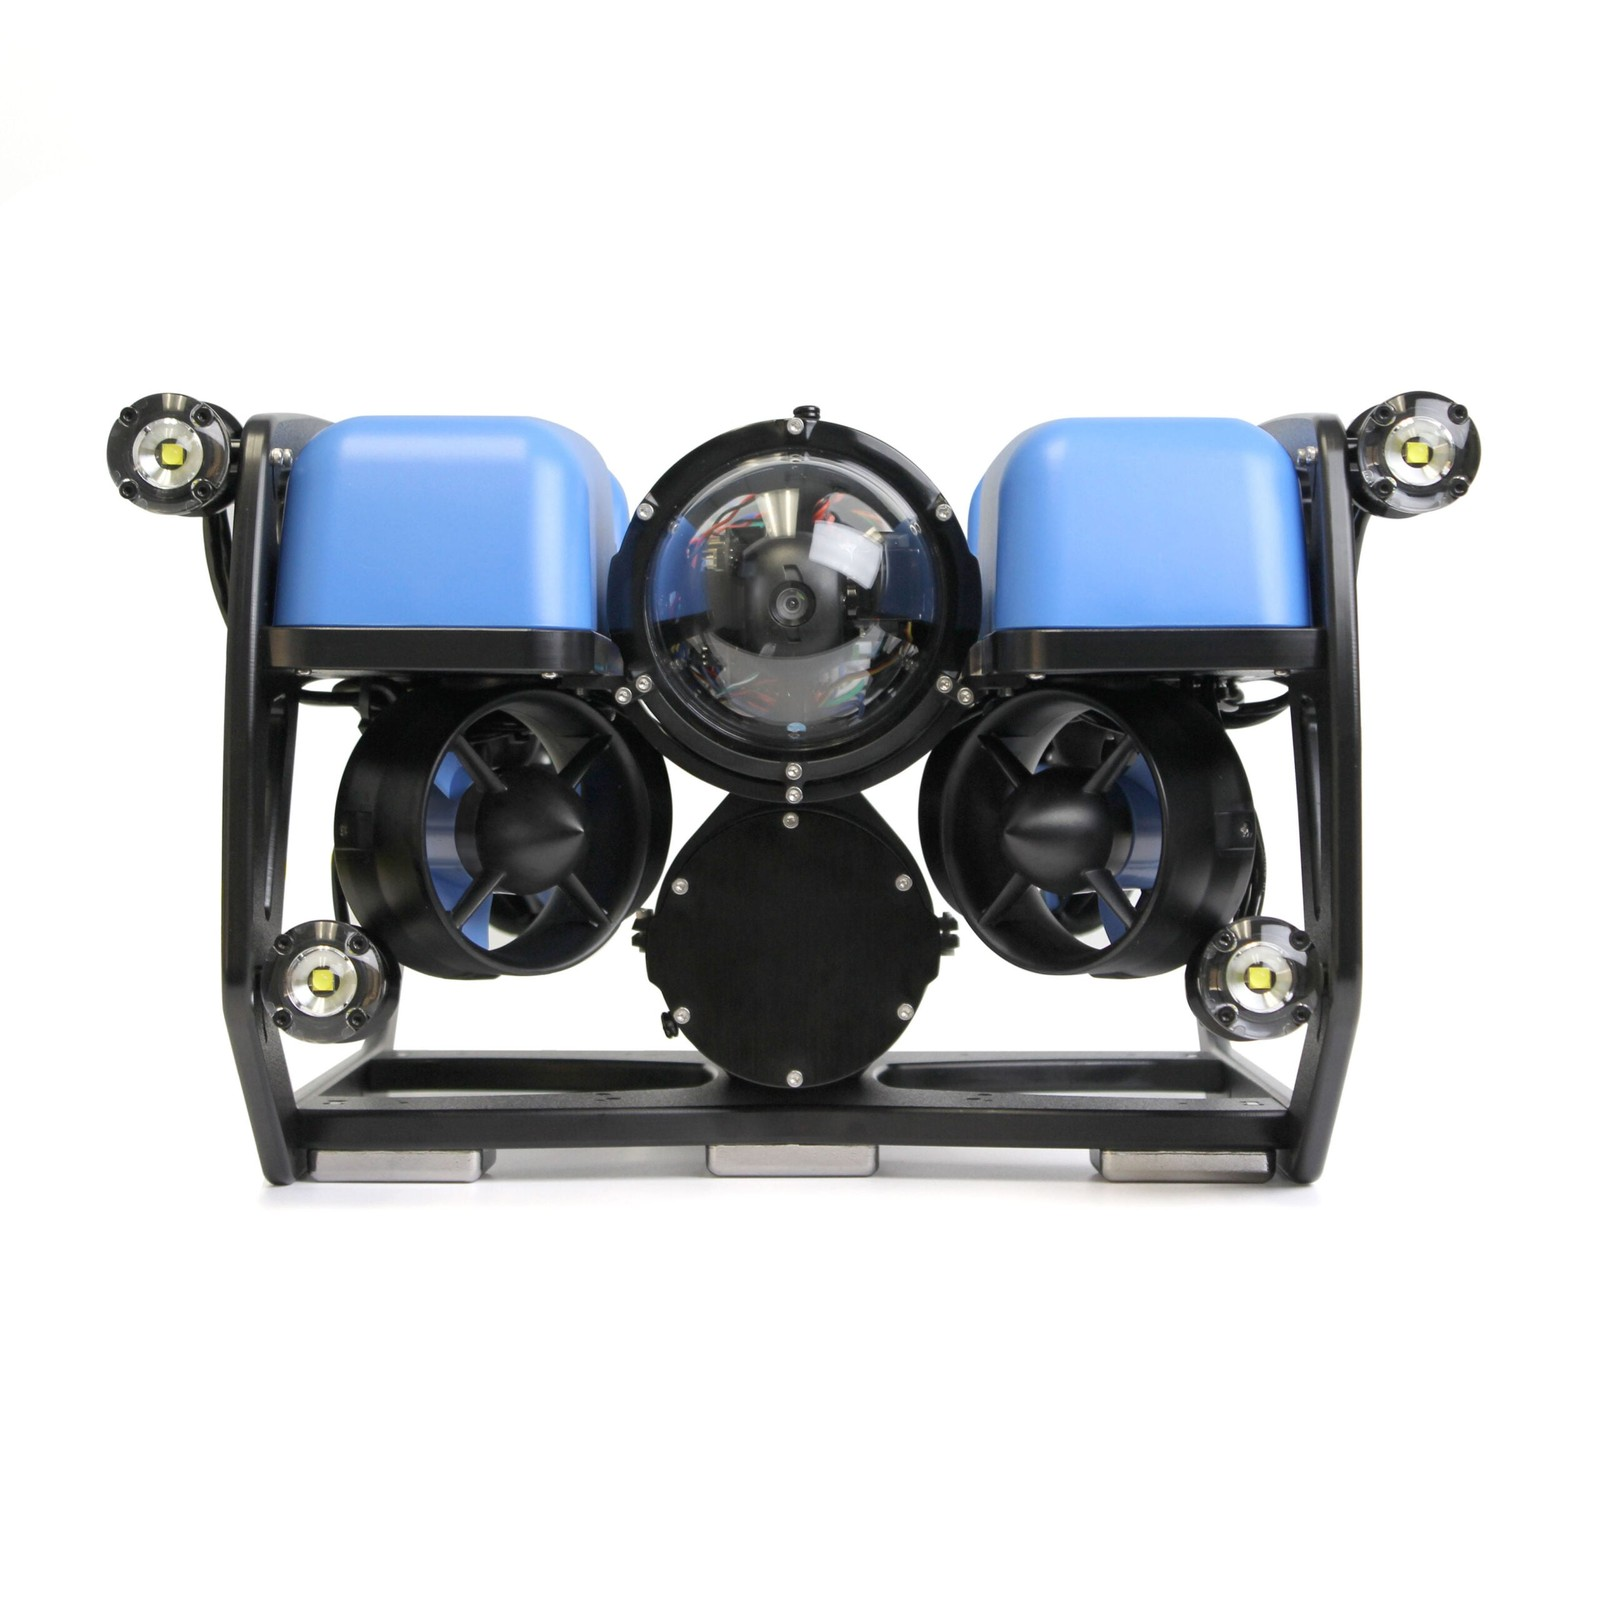
\includegraphics[height=2cm, keepaspectratio]{bluerov2.jpg}\\
        \vspace{0.2em}
        \tech{ROV}\\
        \tiny\textbf{BlueRobotics BlueROV2}\\
        \textit{Télé-opéré filaire}
      \end{center}
      \tiny
      6 DDL, stationnaire fin, inspection vidéo, prélèvements.
    \end{column}

    \begin{column}{0.19\textwidth}
      \begin{center}
        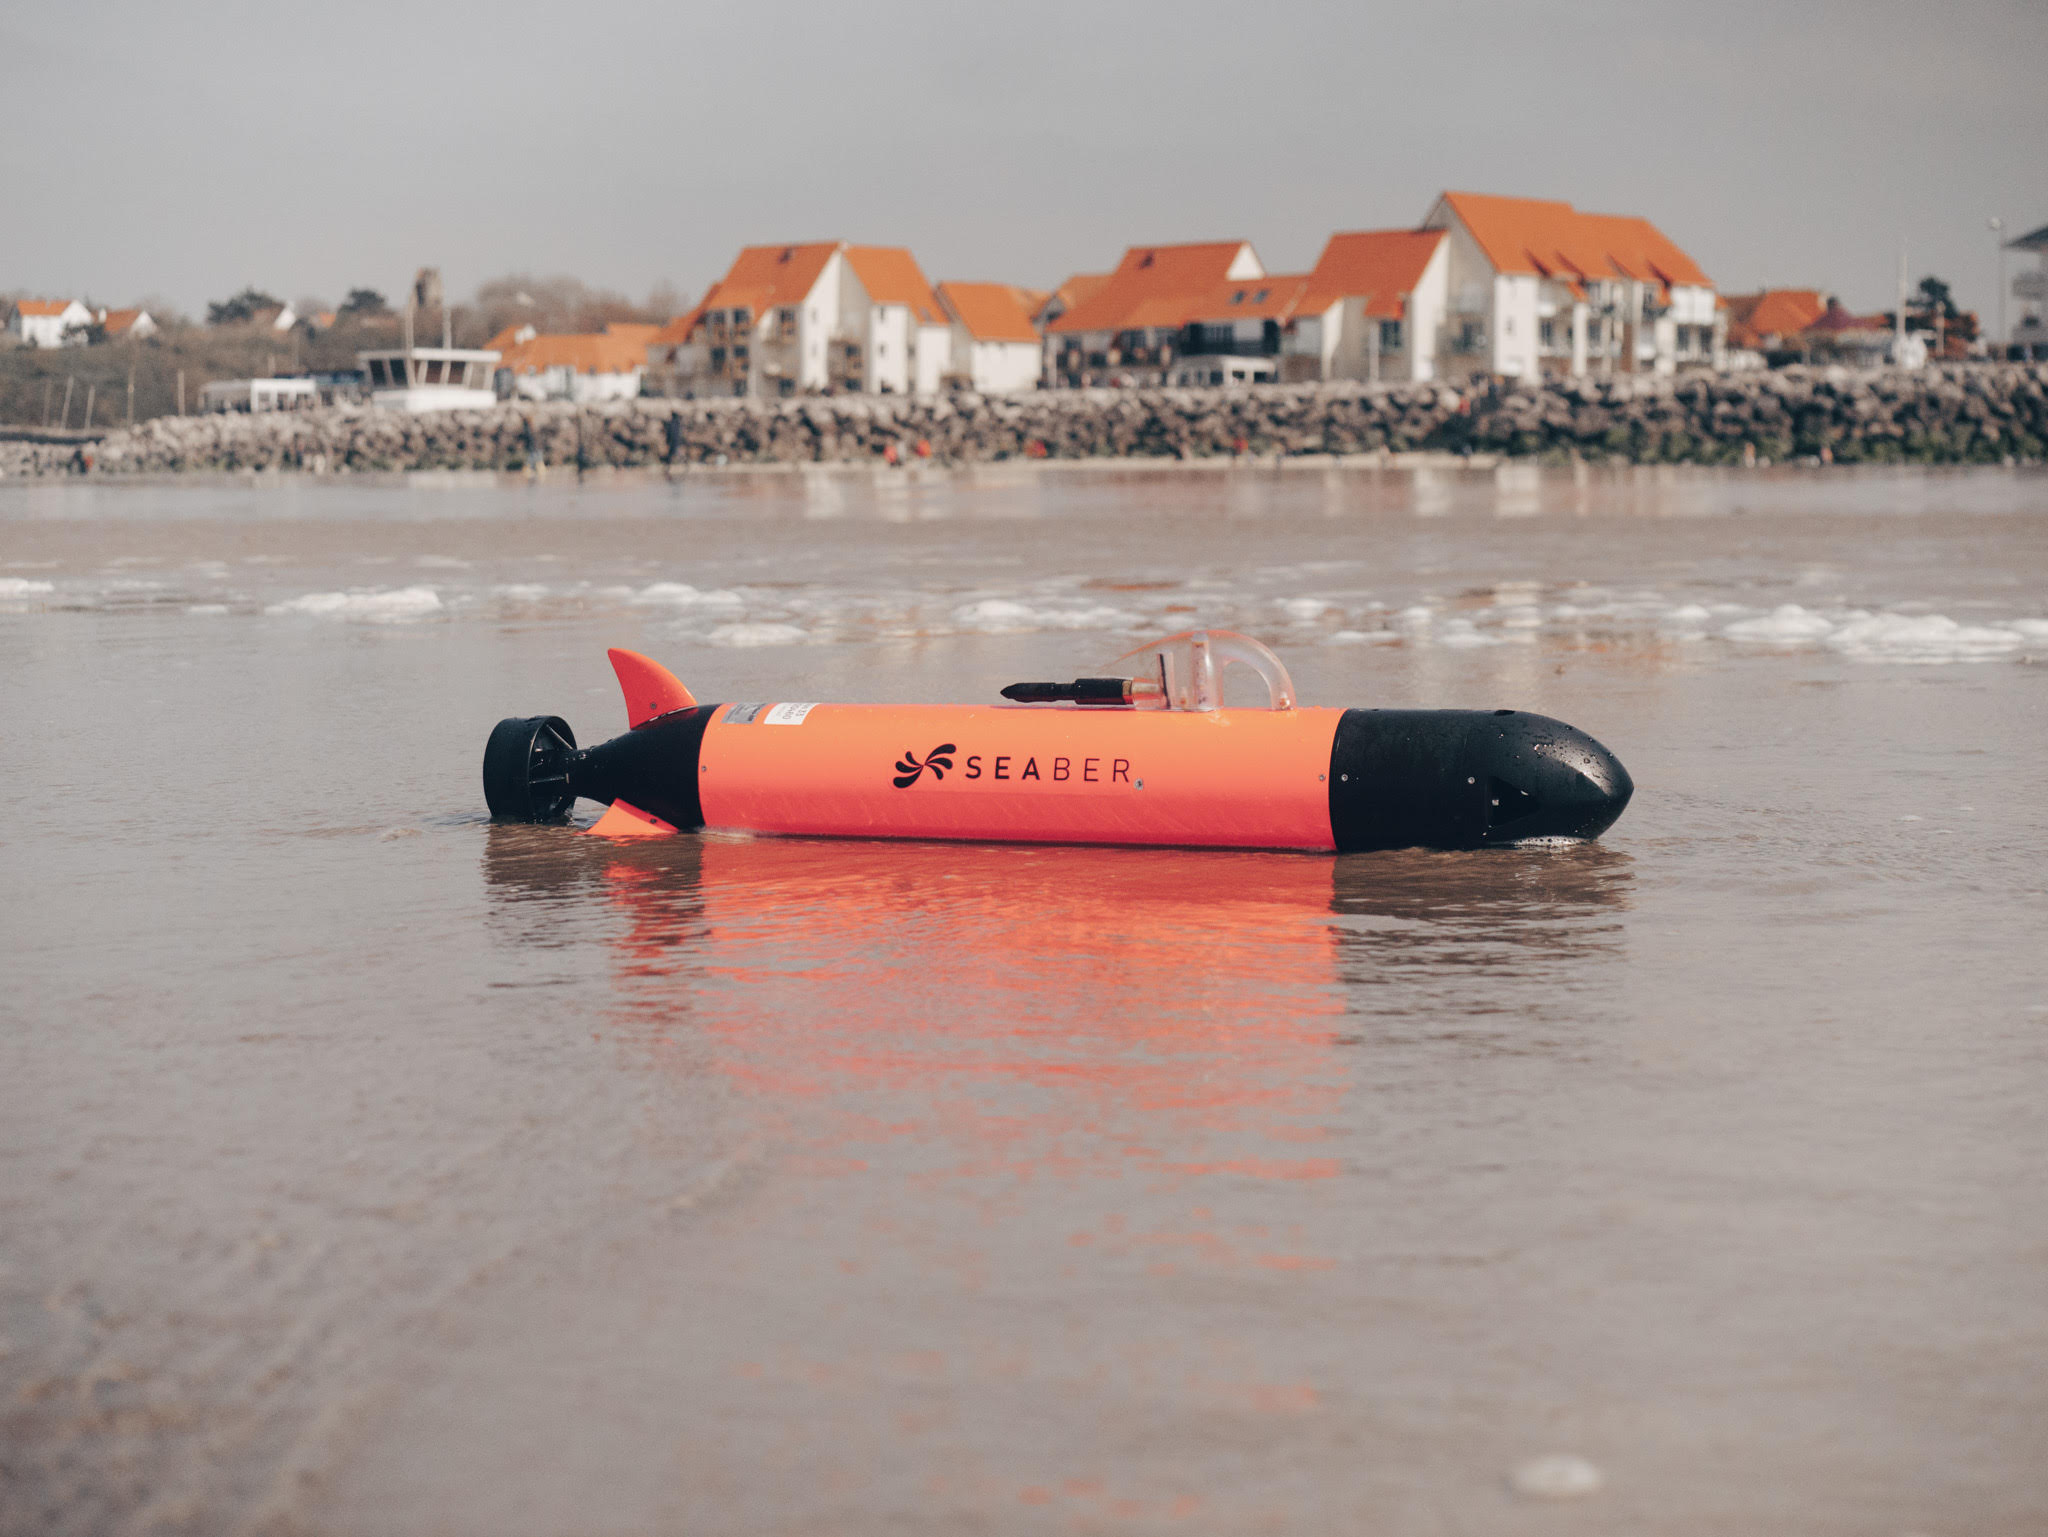
\includegraphics[height=2cm, keepaspectratio]{seaber_yuco.jpg}\\
        \vspace{0.2em}
        \tech{AUV}\\
        \tiny\textbf{Seaber YUCO}\\
        \textit{Autonome propulsé}
      \end{center}
      \tiny
      Transit $3\text{--}6\,\text{kts}$, profils yo-yo CTD, sonar latéral.
    \end{column}

    \begin{column}{0.19\textwidth}
      \begin{center}
        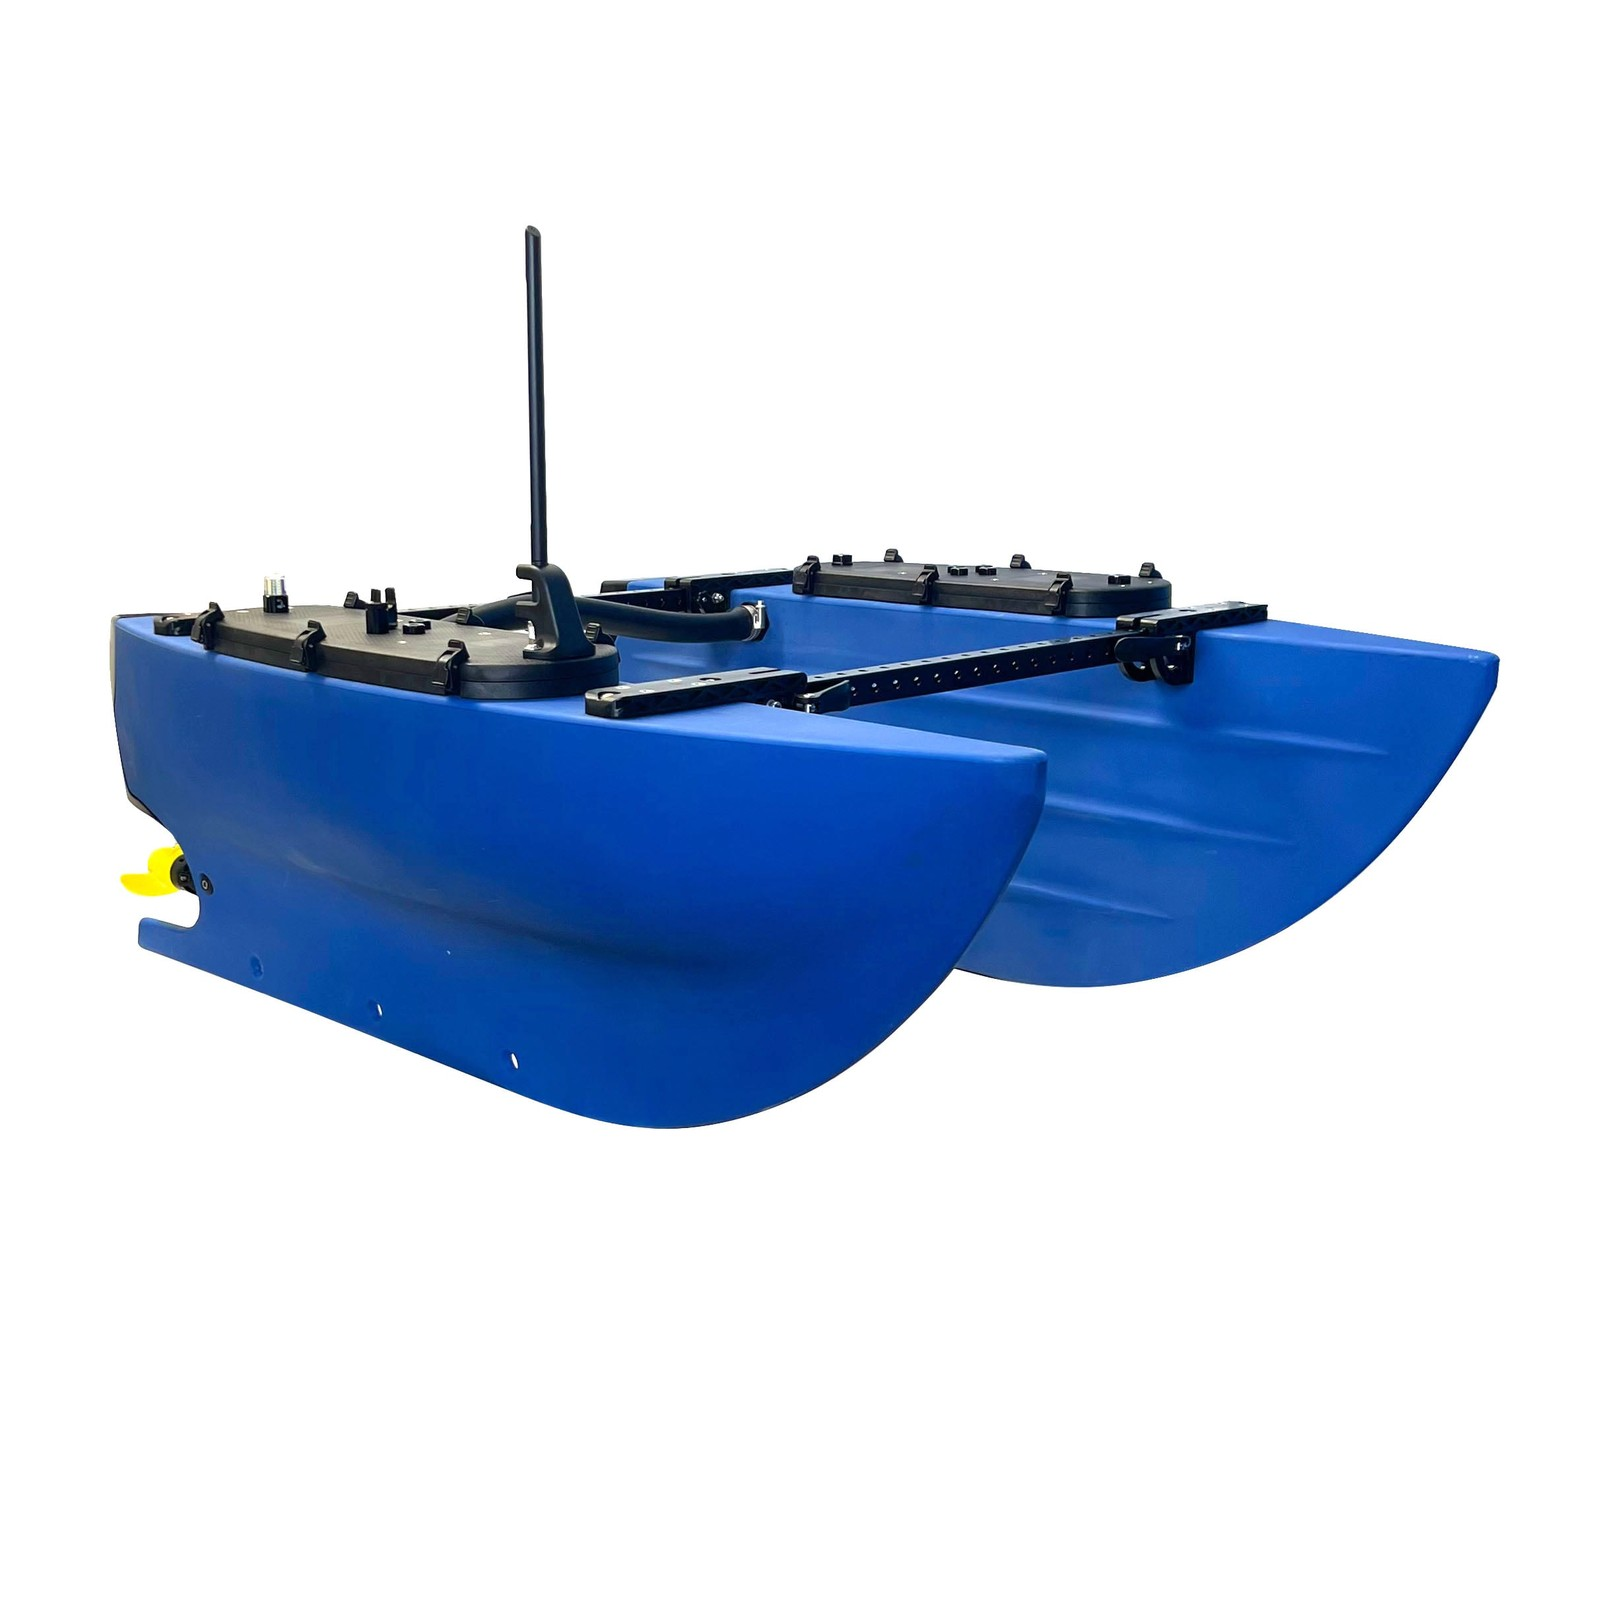
\includegraphics[height=2cm, keepaspectratio]{blueboat.jpg}\\
        \vspace{0.2em}
        \tech{ASV / USV}\\
        \tiny\textbf{BlueRobotics BlueBoat}\\
        \textit{Surface autonome}
      \end{center}
      \tiny
      GNSS, inspection de surface, bathymétrie fauchée mono/multi.
    \end{column}

    \begin{column}{0.21\textwidth}
      \begin{center}
        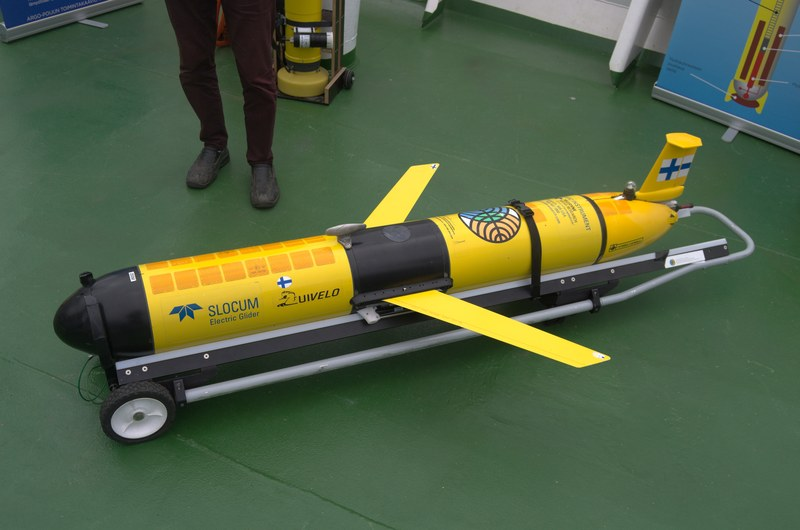
\includegraphics[height=2cm, keepaspectratio]{slocum_glider_clean.jpg}\\
        \vspace{0.2em}
        \succw{Glider}\\
        \tiny\textbf{Teledyne Slocum}\\
        \textit{Flottabilité variable}
      \end{center}
      \tiny
      Endurance plusieurs mois, sonde CTD, capteurs biochimiques, profils dents de scie transocéaniques.
    \end{column}

    \begin{column}{0.20\textwidth}
      \begin{center}
        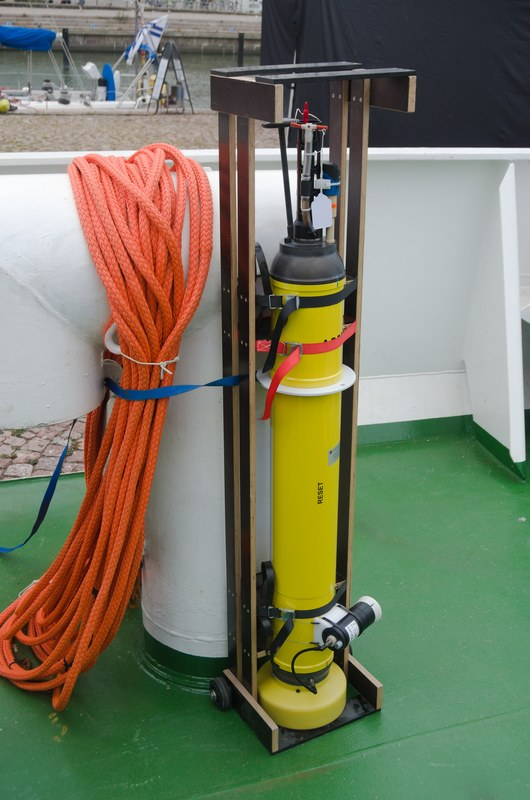
\includegraphics[height=2cm, keepaspectratio]{argo_float_clean.jpg}\\
        \vspace{0.2em}
        \alertw{Bouée Argo}\\
        \tiny\textbf{Teledyne Apex}\\
        \textit{Lagrangien profilant}
      \end{center}
      \tiny
      Cycles 10 jours, dérive $1000\,\text{m}$, 4 à 6 ans autonomie, sondes CTD, analyse des courants, capteurs biochimiques.
    \end{column}
  \end{columns}
\end{frame}

\begin{frame}{1.1b Zoom sur les Micro-AUVs : L'Exemple Seaber YUCO}
  \begin{columns}[c]
    \begin{column}{0.44\textwidth}
      \begin{center}
        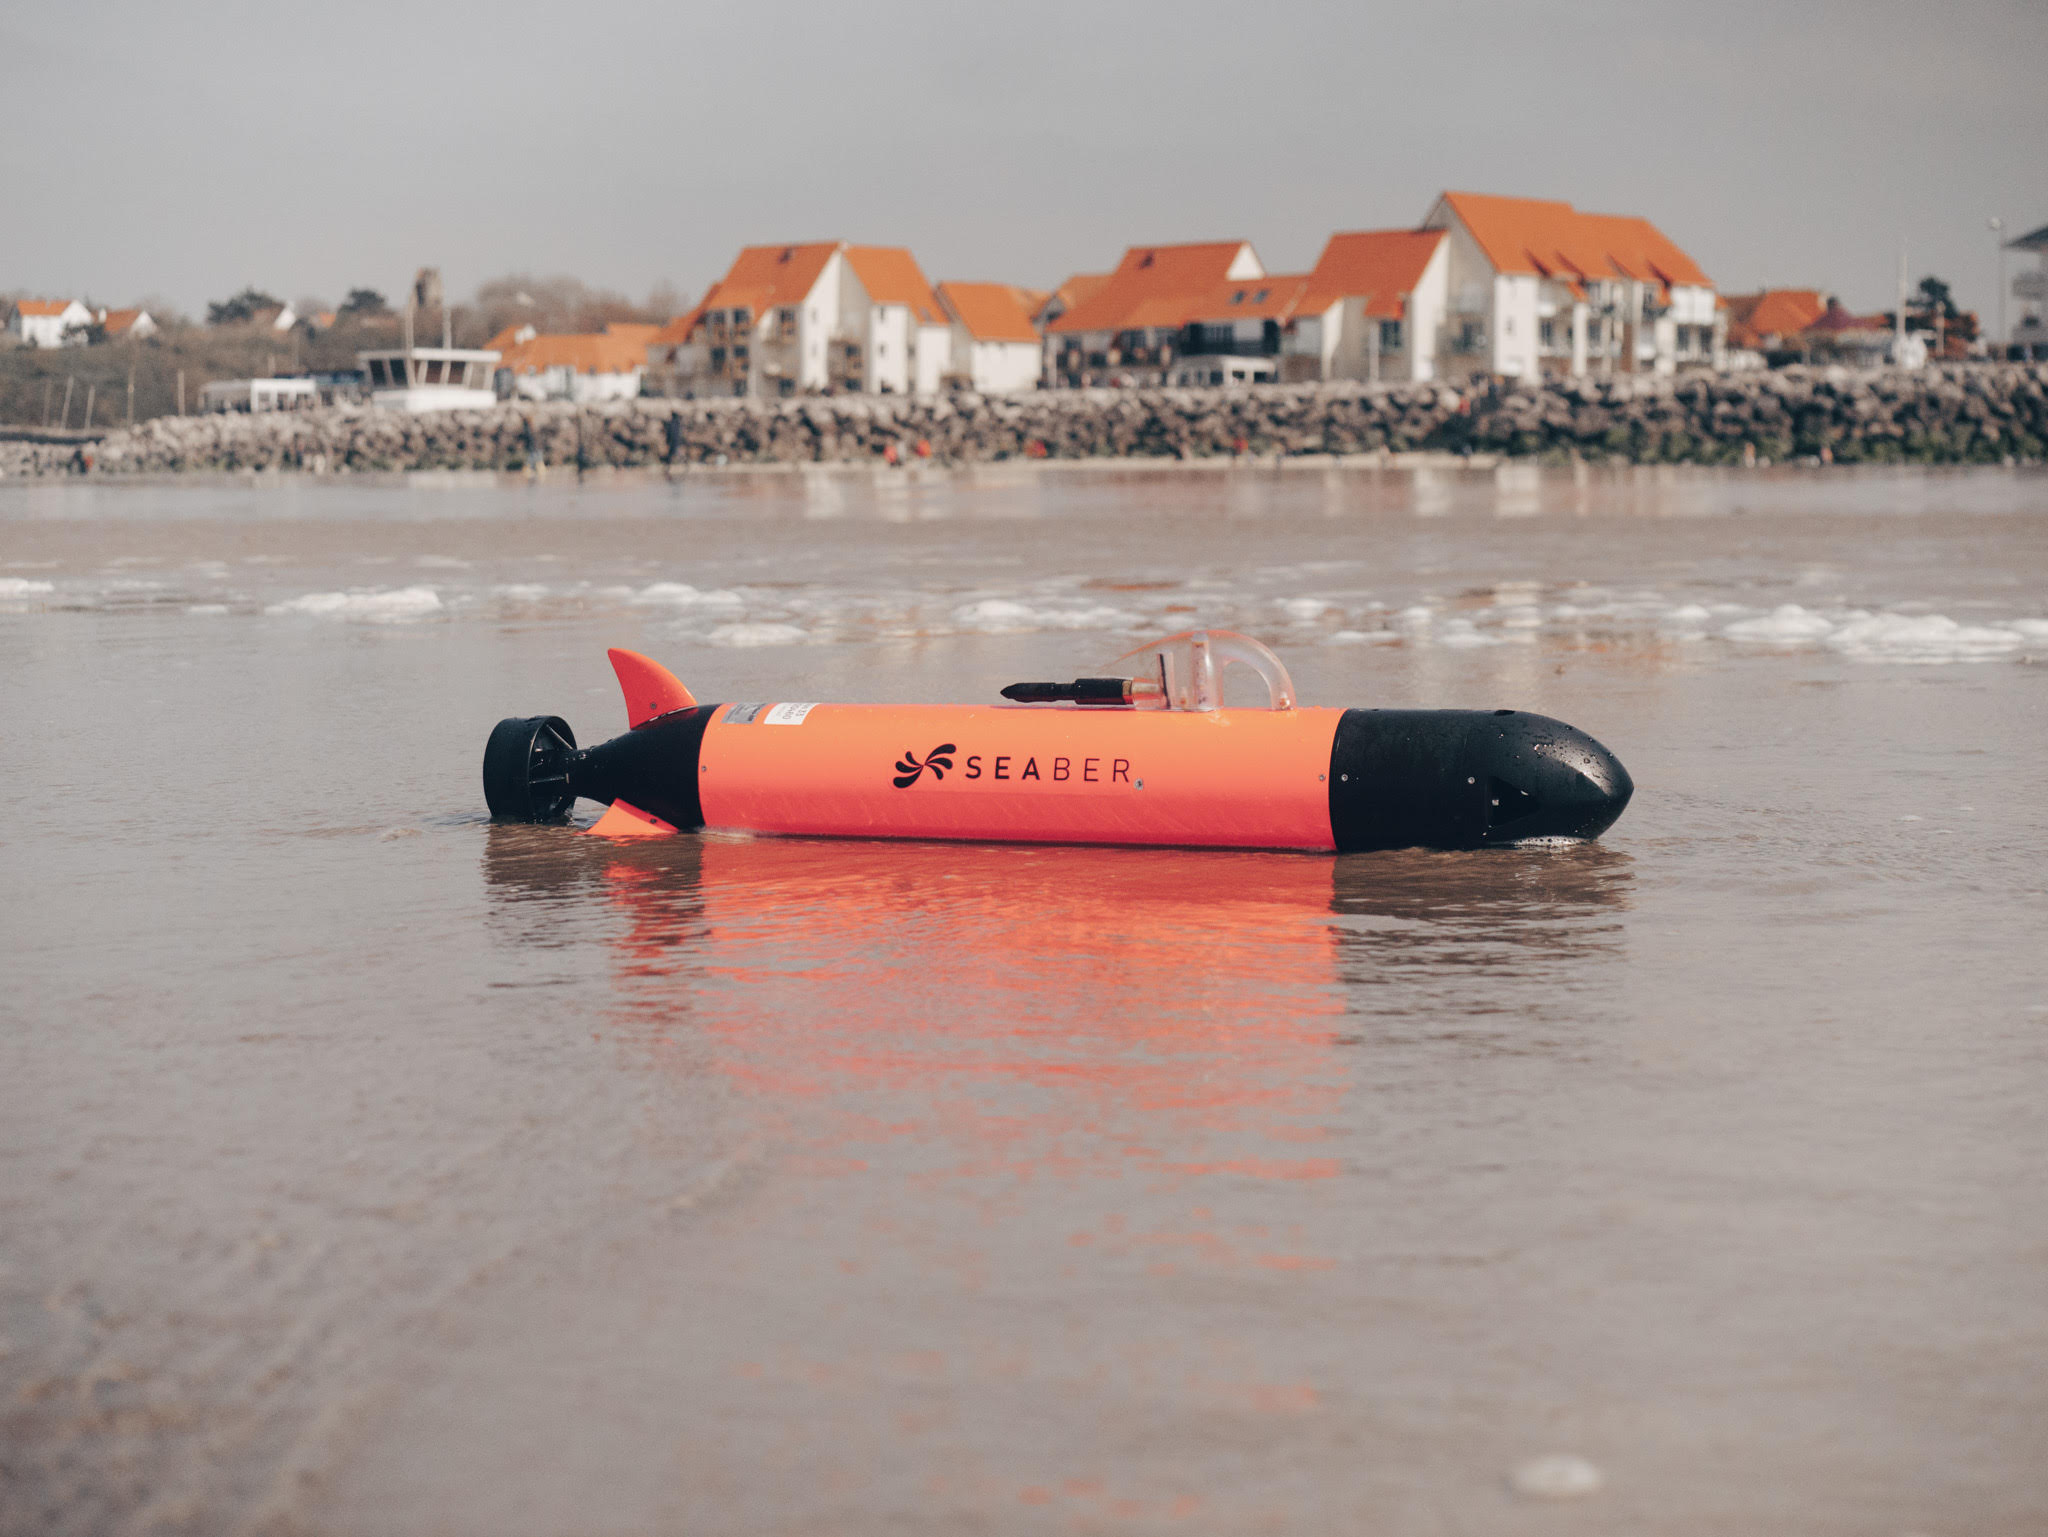
\includegraphics[width=\textwidth, height=3.0cm, keepaspectratio]{seaber_yuco.jpg}\\
        \vspace{0.2em}
        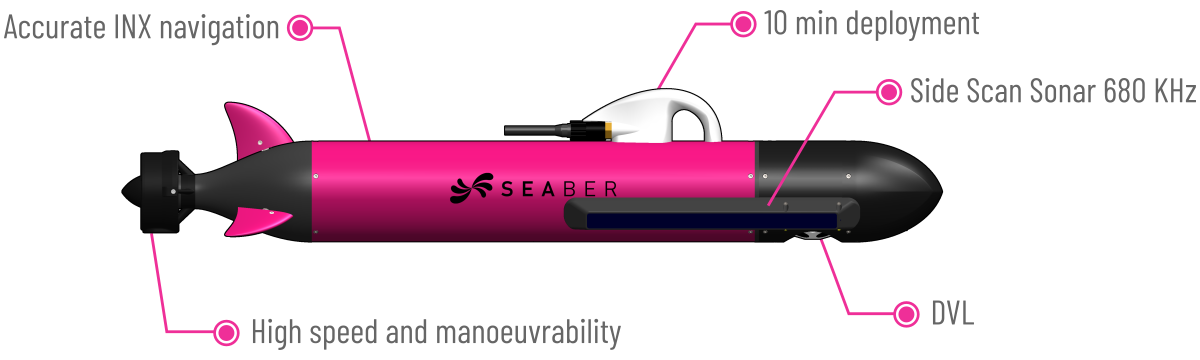
\includegraphics[width=\textwidth, height=1.45cm, keepaspectratio]{seaber_yuco_diagram.png}\\
        \vspace{0.1em}
        \scriptsize\textbf{Micro-AUV Seaber YUCO} (Lorient, France)\\
        \tiny\textit{Longueur $1\,\text{m}$ $\cdot$ Masse $10\,\text{kg}$ $\cdot$ Immersion $300\,\text{m}$ $\cdot$ Vitesse $3\text{--}6\,\text{kts}$}
      \end{center}
    \end{column}

    \begin{column}{0.54\textwidth}
      \begin{block}{\tech{La Révolution du Micro-AUV Côtier}}
        \scriptsize
        \begin{itemize}
          \item \textbf{Démocratisation} : déployable \succw{par 1 seul opérateur} (caisse de transport rigide compacte $<15\,\text{kg}$ tout compris).
          \item \textbf{Navigation inertielle INX©} : haute précision sans balisage acoustique lourd (LBL). Recalage fond par DVL-A50.
          \item \textbf{Autonomie \& Transit} : 8 à 10 h d'endurance, propulsion par hélice carénée et gouvernes arrière.
        \end{itemize}
      \end{block}

      \begin{exampleblock}{\tech{Déclinaisons Scientifiques \& Payloads}}
        \scriptsize
        \begin{itemize}
          \item \textbf{YUCO-CTD} : sonde Seabird/RBR en vol ondulant (\textit{yo-yo}).
          \item \textbf{YUCO-Scan} : sonar latéral ($680\,\text{kHz}$) pour cartographie benthique.
          \item \textbf{YUCO-Carrier / PAM} : capteurs sur mesure et écoute acoustique.
        \end{itemize}
      \end{exampleblock}
    \end{column}
  \end{columns}
\end{frame}

\begin{frame}{1.1b2 Zoom sur les Planeurs Sous-Marins : L'Exemple Slocum Glider}
  \begin{columns}[c]
    \begin{column}{0.42\textwidth}
      \begin{center}
        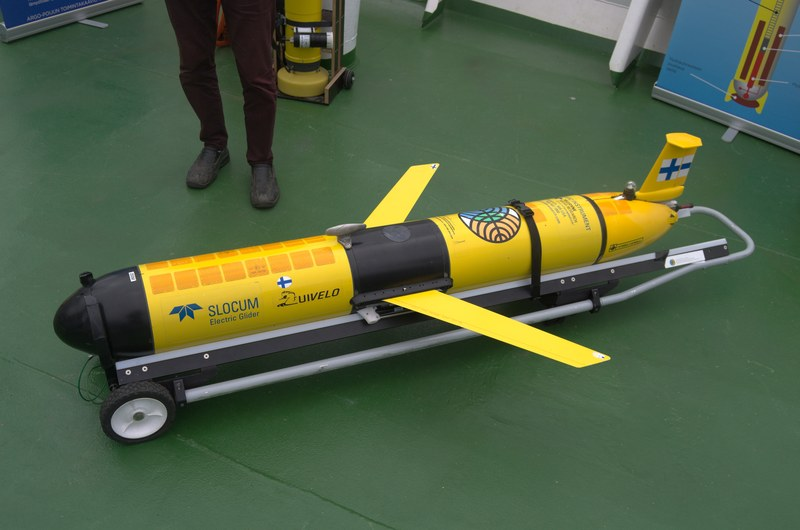
\includegraphics[width=\textwidth, height=3.6cm, keepaspectratio]{slocum_glider_clean.jpg}\\
        \vspace{0.2em}
        \small\textbf{Teledyne Webb Slocum G3 Glider}\\
        \scriptsize\textit{Planeur sous-marin océanographique autonome}
      \end{center}
    \end{column}

    \begin{column}{0.56\textwidth}
      \begin{block}{\succw{Principe de Propulsion par Flottabilité Variable}}
        \scriptsize
        \begin{itemize}
          \item \textbf{Moteur de flottabilité} : une pompe hydraulique transfère de l'huile entre un réservoir interne et une vessie externe.
          \item \textbf{Conversion d'Archimède en poussée} : la variation de volume fait couler ou flotter l'engin ; les ailes fixes transforment ce mouvement vertical en vitesse horizontale (trajectoire en dents de scie).
          \item \textbf{Pas d'actionneurs en continu} : très faible consommation électrique ($\approx 1\text{--}2\,\text{W}$ moyen), quasi-silencieux (idéal acoustique passive).
        \end{itemize}
      \end{block}

      \begin{exampleblock}{\tech{Caractéristiques Techniques \& Missions}}
        \scriptsize
        \begin{itemize}
          \item \textbf{Vitesse} : $0.5\text{--}1\,\text{n\oe ud}$ ($0.25\text{--}0.5\,\text{m/s}$) $\cdot$ \textbf{Immersion} : $200\,\text{m}$ à $1000\,\text{m}$ ($6000\,\text{m}$ Deep).
          \item \textbf{Autonomie} : \succw{Plusieurs semaines à 1 an} ($>4\,000\text{--}10\,000\,\text{km}$).
          \item \textbf{Surfaçage \& Comms} : antenne dans l'empennage relevé en surface pour recalage GNSS et transmission satellite Iridium bidirectionnelle.
          \item \textbf{Capteurs} : CTD, oxygène dissous ($O_2$), chlorophylle, turbidité, écoute acoustique passive pour cétacés.
        \end{itemize}
      \end{exampleblock}
    \end{column}
  \end{columns}
\end{frame}

\begin{frame}{1.1b3 Zoom sur les Flotteurs Profilants Dérivants : Le Réseau Argo}
  \begin{columns}[c]
    \begin{column}{0.40\textwidth}
      \begin{center}
        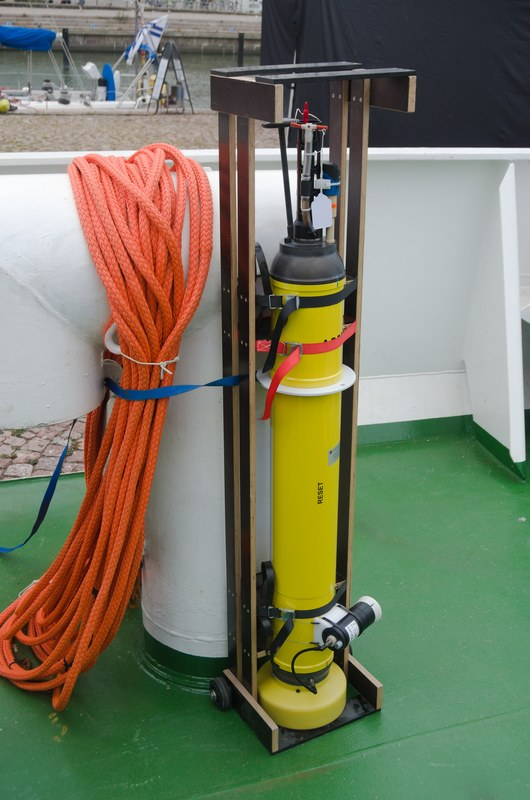
\includegraphics[width=\textwidth, height=4.5cm, keepaspectratio]{argo_float_clean.jpg}\\
        \vspace{0.2em}
        \small\textbf{Flotteur Profilant Dérivant (Argo)}\\
        \scriptsize\textit{Modèles Provor / Arvor (NKE/Ifremer) ou Apex / Navis}
      \end{center}
    \end{column}

    \begin{column}{0.58\textwidth}
      \begin{block}{\alertw{Principe de Fonctionnement}}
        \scriptsize
        \begin{enumerate}
          \item \textbf{Plongée profonde} : descente jusqu'à $2000\,\text{m}$ (ou $4000\text{--}6000\,\text{m}$ pour Deep Argo).
          \item \textbf{Remontée profilante} : ascension continue vers la surface en enregistrant la colonne d'eau (température, salinité, pression).
          \item \textbf{Surfaçage \& Télétransmission} : transmission des profils par satellite (Iridium), positionnement GPS, puis purge et nouvelle plongée.
        \end{enumerate}
      \end{block}

      \begin{exampleblock}{\tech{Caractéristiques Clés \& Impact Scientifique}}
        \scriptsize
        \begin{itemize}
          \item \textbf{Autonomie} : \succw{4 à 6 ans en mer} ($\approx 150\text{--}250$ cycles complets) sur piles Lithium.
          \item \textbf{Réseau mondial} : \textbf{$\approx 4\,000$ flotteurs actifs} en permanence dans tous les océans (données ouvertes en temps réel).
          \item \textbf{Payload métrologique} : sonde CTD haute précision (Seabird SBE41CP), capteurs BGC-Argo ($O_2$, pH, nitrates, Chl-a).
          \item \textbf{Applications} : climatologie globale, bilan thermique océanique, calibration altimétrie spatiale (Copernicus, SWOT).
        \end{itemize}
      \end{exampleblock}
    \end{column}
  \end{columns}
\end{frame}

\begin{frame}{1.1c Ordres de Grandeur des Coûts d'Acquisition (Porteurs $\approx 1\,\text{m}$)}
  \scriptsize
  \begin{table}[h]
    \centering
    \begin{tabularx}{\textwidth}{l p{2.6cm} p{2.2cm} p{2.8cm} X}
      \toprule
      \textbf{Famille} & \textbf{Modèle Réf.} & \textbf{Porteur Nu / Base} & \textbf{Équipé Recherche} & \textbf{Alternative Ind. / Défense} \\
      \midrule
      \rowcolor{OceanGray}
      \tech{ROV} \tiny(Filaire) & BlueROV2 Heavy \tiny(BlueRobotics, US) & $\approx \mathbf{4{,}5\text{--}6\,\text{k€}}$ & $\approx \mathbf{8\text{--}15\,\text{k€}}$ \tiny(Fathom $150\,\text{m}$, console, pince, DVL opt.) & $>40\text{--}120\,\text{k€}$ \tiny(VideoRay Defender, Deep Trekker Pivot) \\
      \tech{ASV / USV} \tiny(Surface) & BlueBoat \tiny(BlueRobotics, US) & $\approx \mathbf{3{,}5\text{--}5\,\text{k€}}$ & $\approx \mathbf{7\text{--}18\,\text{k€}}$ \tiny(GNSS, sondeur Ping ou MBES Cerulean) & $>50\text{--}250\,\text{k€}$ \tiny(OceanAlpha SL40, Exail DriX, Maritime Robotics Otter) \\
      \rowcolor{OceanGray}
      \tech{Micro-AUV} & Seaber YUCO \tiny(Seaber, FR) & $\approx \mathbf{25\text{--}35\,\text{k€}}$ \tiny(Carrier intégration) & $\approx \mathbf{35\text{--}75\,\text{k€}}$ \tiny(YUCO-CTD / Scan avec DVL et acoustique) & $>150\text{--}500\,\text{k€}$ \tiny(Gavia, REMUS 100, Exail A18) \\
      \bottomrule
    \end{tabularx}
  \end{table}

  \vspace{0.2em}
  \begin{columns}[T]
    \begin{column}{0.48\textwidth}
      \begin{block}{\tech{Pourquoi de Tels Écarts de Prix ?}}
        \begin{itemize}
          \item Les briques open-source (ArduSub/ArduRover) et composants modulaires divisent le coût d'accès par un facteur $3$ à $10\times$.
          \item Les systèmes industriels/défense intègrent une certification militaire, redondance totale et SAV sur site à coût élevé.
        \end{itemize}
      \end{block}
    \end{column}

    \begin{column}{0.50\textwidth}
      \begin{block}{\succw{Impact Budgétaire de la Charge Utile}}
        \begin{itemize}
          \item Les capteurs scientifiques (DVL-A50 : $\approx 7\,\text{k€}$, sondeur MBES Cerulean : $\approx 8\,\text{k€}$, sonde CTD calibrée : $\approx 8\text{--}15\,\text{k€}$) représentent souvent \succw{$50\%$ à $70\%$ du coût global} du vecteur !
          \item Penser aux accessoires : ombilicaux, valises étanches, batteries de rechange, consoles terrain durcies.
        \end{itemize}
      \end{block}
    \end{column}
  \end{columns}
\end{frame}

\begin{frame}{1.1d Écosystème Industriel : Constructeurs Clés \& Revendeurs Français}
  \begin{columns}[T]
    \begin{column}{0.50\textwidth}
      \begin{block}{\tech{Constructeurs Mondiaux ($\approx 1\,\text{m}$ / Portables)}}
        \scriptsize
        \begin{itemize}
          \item \textbf{BlueRobotics} \textit{(USA)} : leader matériel modulaire open-source (BlueROV2, BlueBoat, T200, WetLink, BlueOS).
          \item \textbf{Seaber} \textit{(France - Lorient)} : pionnier des micro-AUVs côtiers légers (gamme YUCO $<10\,\text{kg}$, navigation INX©).
          \item \textbf{RTSYS} \textit{(France - Lorient)} : micro-AUVs acoustiques (NemoSens), modems et balises sous-marines.
          \item \textbf{Deep Trekker} \textit{(Canada)} : ROVs d'inspection robustes (DTG3, Pivot, Revolution).
          \item \textbf{Chasing / QYSEA} \textit{(Chine)} : ROVs d'inspection compacts légers (Chasing M2 Pro, Fifish V6).
          \item \textbf{Water Linked} \textit{(Norvège)} : capteurs acoustiques miniaturisés (DVL-A50, Underwater GPS USBL).
        \end{itemize}
      \end{block}
    \end{column}

    \begin{column}{0.48\textwidth}
      \begin{block}{\succw{Revendeurs \& Intégrateurs en France}}
        \scriptsize
        \textit{Canaux marchés publics CNRS/Univ (Chorus Pro, support \& SAV) :}
        \begin{itemize}
          \item \textbf{SyERA} \textit{(Belgentier / Toulon)} : distributeur officiel BlueRobotics, support, durcissement et personnalisations R\&D/défense.
          \item \textbf{ROV Expert} \textit{(Béziers)} : distributeur majeur BlueRobotics (Top 5 mondial), kits montés, pièces, intégration capteurs \& SAV.
          \item \textbf{Subsea Tech} \textit{(Marseille)} : distributeur BlueRobotics, intégrateur sonars/caméras et fabricant USV (SeaCat).
          \item \textbf{MacArtney France} \textit{(Aix-en-Provence)} : connectique SubConn, sonars et instrumentation océanographique.
          \item \textbf{Seaber} \textit{(Lorient)} : constructeur français, vente directe, support recherche et essais en mer.
        \end{itemize}
      \end{block}
    \end{column}
  \end{columns}
\end{frame}

\begin{frame}{1.2 Anatomie d'une Plateforme de Recherche : Le BlueROV2}
  \begin{columns}[c]
    \begin{column}{0.45\textwidth}
      \begin{center}
        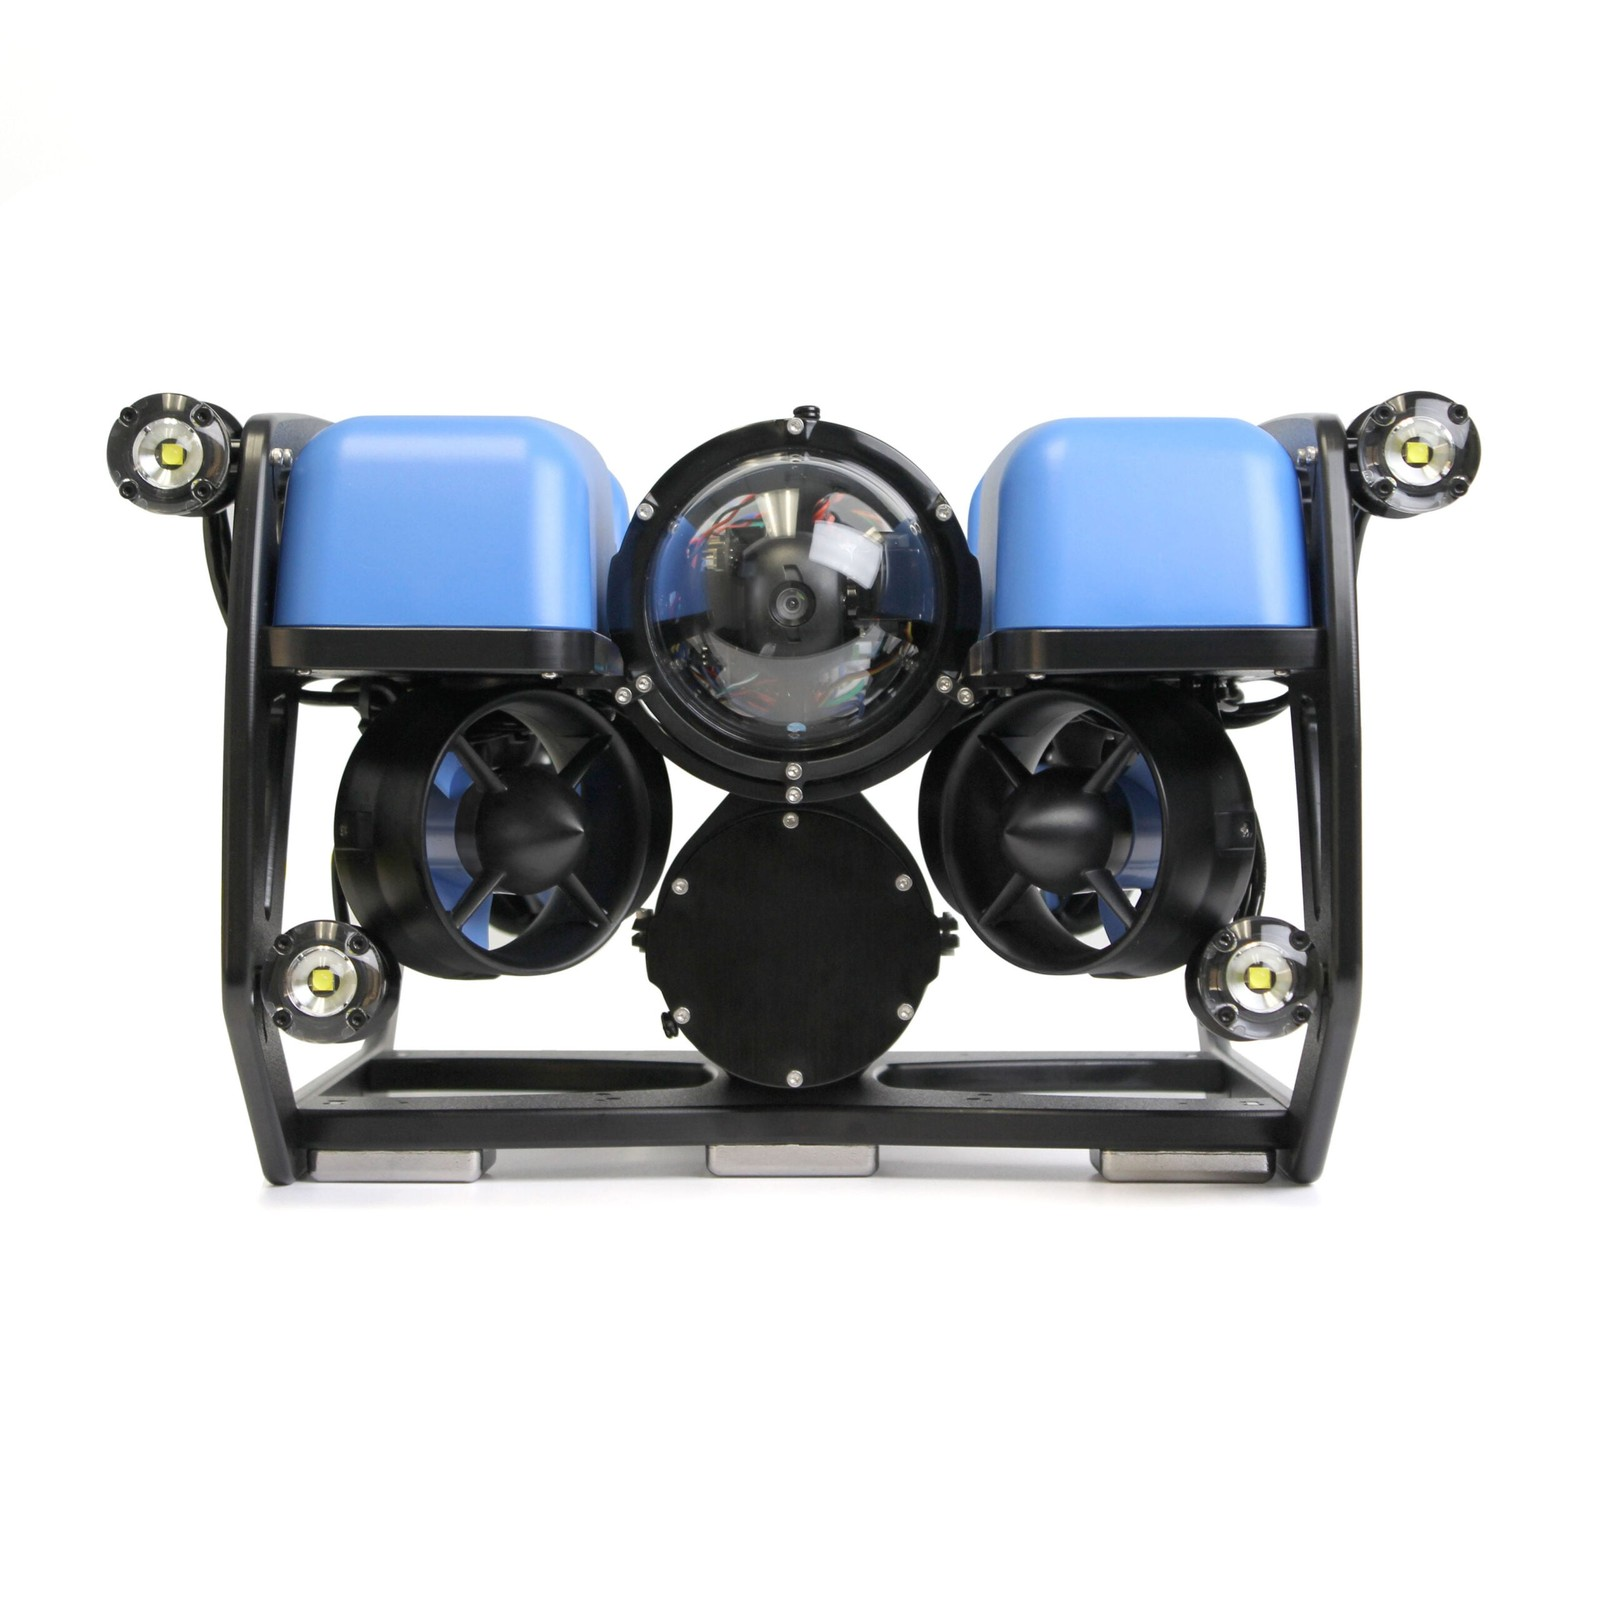
\includegraphics[width=\textwidth, height=4.2cm, keepaspectratio]{bluerov2.jpg}\\
        \vspace{0.2em}
        \small\textbf{BlueROV2} (BlueRobotics)\\
        \scriptsize\textit{Châssis modulaire PEHD, 8 propulseurs vectorisés, double caisson étanche}
      \end{center}
    \end{column}

    \begin{column}{0.53\textwidth}
      \begin{block}{\tech{Architecture Matérielle Découplée}}
        \scriptsize
        \begin{itemize}
          \item \textbf{Caisson Électronique (Tube 4")} : RPi 4/5, carte Navigator, modem Fathom-X, \succw{caméra Low-Light HD sur nacelle tilt}.
          \item \textbf{Caisson Batterie (Tube 3")} : Li-ion 4S $14.8\,\text{V}$ $18\text{Ah}$, interrupteur étanche \& fusible.
          \item \textbf{Capteurs de Sûreté Véhicule} : \alertw{SOS Leak Sensors} (détection fuite fond de tubes) \& capteur de dépression interne.
          \item \textbf{Capteurs \& Indicateurs de Mission} : Pression/profondeur \textbf{Bar30}, \succw{projecteurs étanches Lumen ($2\times 1500\,\text{lm}$)}.
          \item \textbf{Actionnement \& Traversées} : 6 à 8 moteurs \textbf{T200}, pénétrateurs \textbf{WetLink} ou connecteurs \textbf{Cobalt/SubConn}.
          \item \textbf{Ombilical} pour téléopération et transfert de données.
        \end{itemize}
      \end{block}
    \end{column}
  \end{columns}
\end{frame}

\begin{frame}{1.2b L'Énergie Embarquée : Pourquoi Enfermer la Batterie ?}
  \begin{columns}[c]
    \begin{column}{0.42\textwidth}
      \begin{center}
        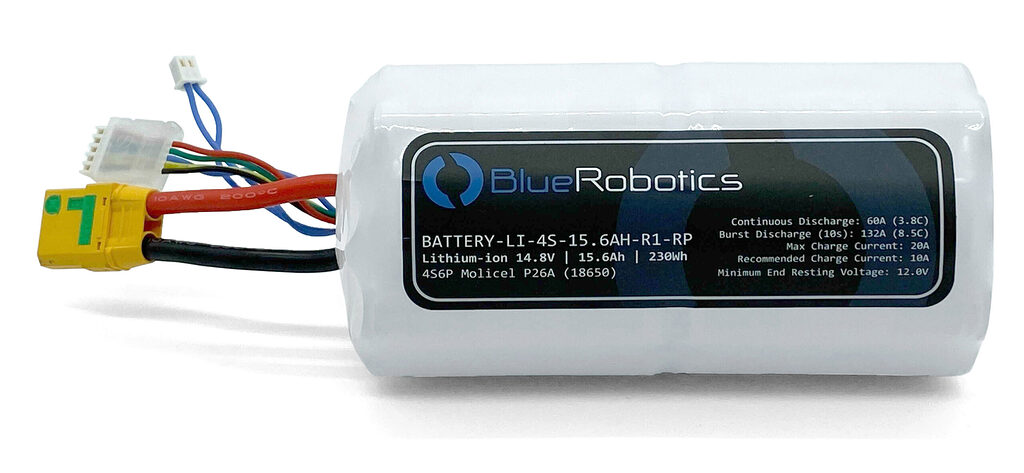
\includegraphics[width=\textwidth, height=2.4cm, keepaspectratio]{battery_pack.jpg}\\
        \vspace{0.2em}
        \tech{Batterie Li-ion 4S ($14.8\,\text{V}$, $15.6\,\text{Ah}$ / $230\,\text{Wh}$)}\\
        \scriptsize\textit{Logée dans un caisson 3" dédié sous le robot}
      \end{center}
      \scriptsize
      \begin{block}{\succw{Avantages de l'Énergie Embarquée}}
        \begin{itemize}
          \item \textbf{Stabilité} : masse lourde ($1.2\,\text{kg}$) au point le plus bas $\rightarrow$ abaisse $G$ et maximise $\overline{BG}$.
          \item \textbf{Courant crête instantané} : jusqu'à \alertw{$132\,\text{A}$} disponibles sans chute de tension.
        \end{itemize}
      \end{block}
    \end{column}

    \begin{column}{0.56\textwidth}
      \textbf{Pourquoi ne pas alimenter en 14.8V depuis la surface ?}
      \scriptsize
      \begin{itemize}
        \item Consommation de 6 à 8 thrusters T200 : $I = \mathbf{30\text{ à }60\,\text{A}}$.
        \item Ombilical fin neutre ($100\text{ à }300\,\text{m}$) : résistance $R \approx 1.5\text{ à }4\,\Omega$.
      \end{itemize}

      \vspace{0.2em}
      \begin{alertblock}{La Chute de Tension Ohmique ($\Delta V = R \cdot I$)}
        \scriptsize
        \[
          \Delta V = 2\,\Omega \times 30\,\text{A} = \mathbf{60\,\text{V}} \quad (\gg 14.8\,\text{V} !)
        \]
        La tension arrivant au robot serait \alertw{négative ou quasi-nulle} ! Les moteurs caleraient instantanément.
      \end{alertblock}

      \begin{alertblock}{Les Pertes Joule Destructrices ($P = R \cdot I^2$)}
        \scriptsize
        \[
          P_{\text{perte}} = 2\,\Omega \times (30\,\text{A})^2 = \mathbf{1800\,\text{W}}
        \]
        L'énergie serait dissipée en pure chaleur dans le câble $\rightarrow$ \alertw{fusion de l'ombilical} !
      \end{alertblock}
    \end{column}
  \end{columns}
\end{frame}

\begin{frame}{1.3 L'Actionnement Réel : Le Propulseur Brushless T200}
  \begin{columns}[c]
    \begin{column}{0.62\textwidth}
      \textbf{Pourquoi le T200 est-il unique ?}
      \scriptsize
      \begin{itemize}
        \item \textbf{Moteur noyé (Flooded)} : l'eau de mer circule librement à l'intérieur $\rightarrow$ \succw{refroidissement direct des bobinages}.
        \item \textbf{Encapsulation résine époxy} : stator surmoulé sous vide.
        \item \textbf{Paliers autolubrifiants PEEK} : zéro roulement métallique.
        \item \textbf{Aimants néodyme scellés} : revêtement époxy anticorrosion.
      \end{itemize}

      \vspace{0.2em}
      \begin{block}{Performances \& Contrôleurs ESC}
        \scriptsize
        \begin{itemize}
          \item Poussée T200 : jusqu'à \textbf{$5.25\,\text{kgf}$} ($14.8\,\text{V}$ / Li-ion 4S).
          \item \tech{Basic ESC (30A)} : $7\text{--}26\,\text{V}$, $50\,\text{A}$ continu, dissipation accrue pour caisson fermé.
          \item \succw{Commande réversible} : PWM bidirectionnel ($1100\,\mu\text{s}$ AR -- $1500\,\mu\text{s}$ Stop -- $1900\,\mu\text{s}$ AV).
        \end{itemize}
      \end{block}
    \end{column}

    \begin{column}{0.35\textwidth}
      \begin{center}
        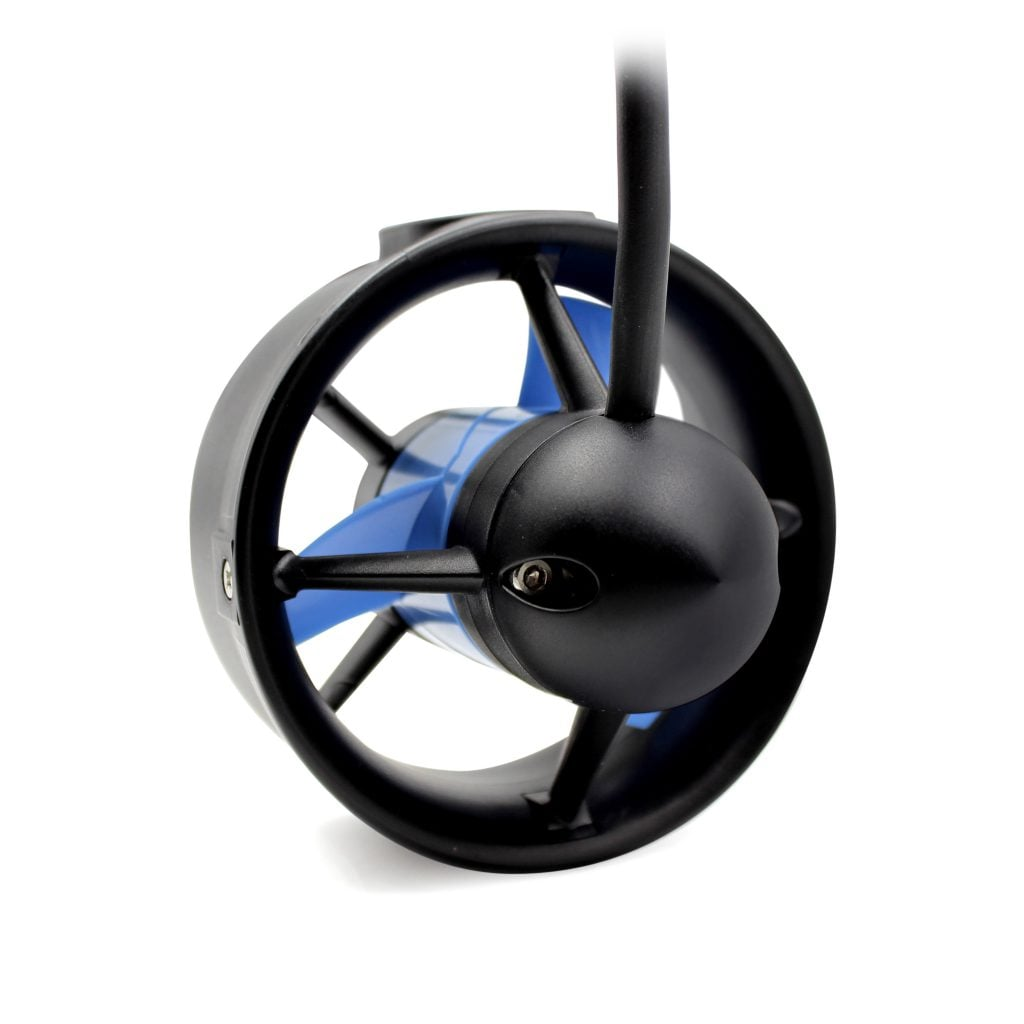
\includegraphics[height=3.2cm, keepaspectratio]{t200_thruster.png}\\
        \vspace{0.2em}
        \footnotesize\textbf{Propulseur T200}\\
        \scriptsize\textit{Stator noyé \& hélice polycarbonate}
      \end{center}
    \end{column}
  \end{columns}
\end{frame}

\begin{frame}{1.3b Panorama des Actionneurs Marins : T200, T500 \& Servos}
  \begin{columns}[T]
    \begin{column}{0.32\textwidth}
      \begin{center}
        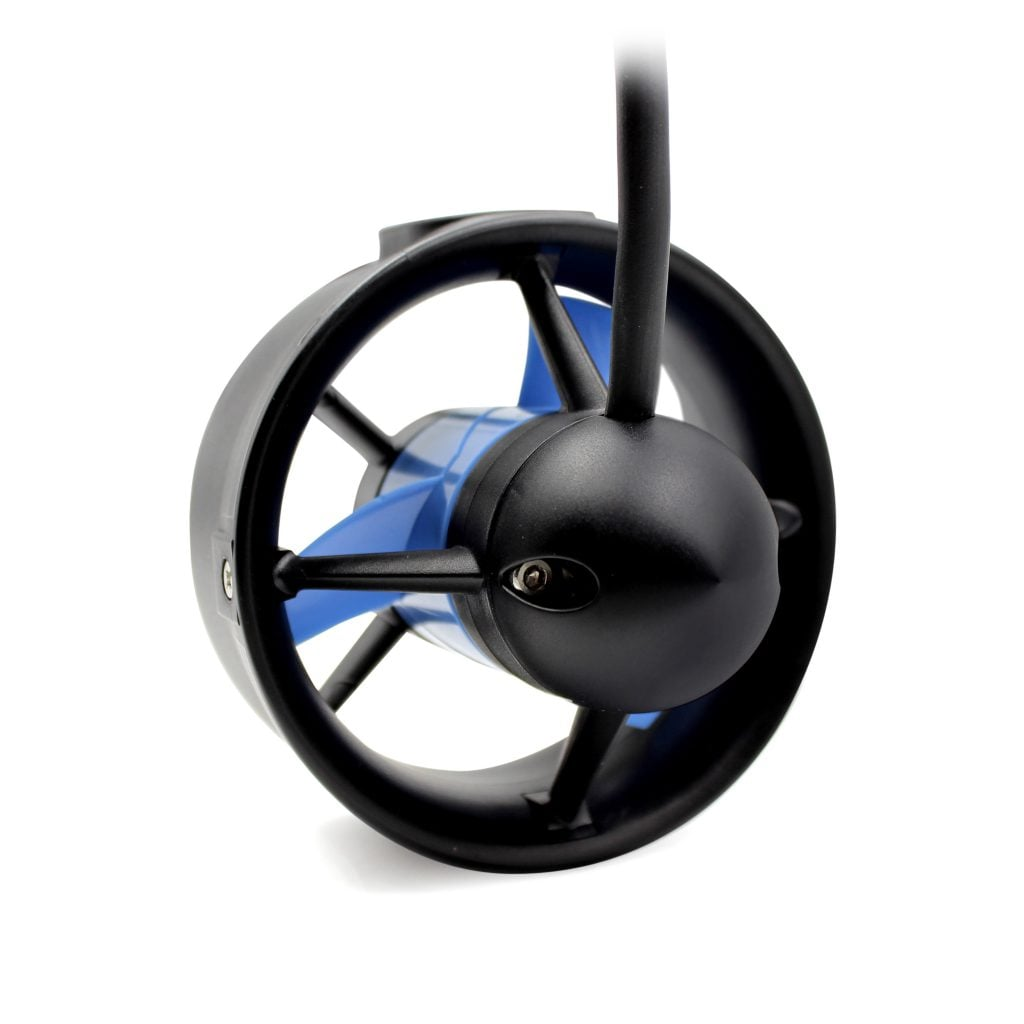
\includegraphics[height=2.3cm, keepaspectratio]{t200_thruster.png}\\
        \vspace{0.2em}
        \tech{T200 Thruster}\\
        \footnotesize\textbf{Standard ROV \& ASV}
      \end{center}
      \scriptsize
      \begin{itemize}
        \item Poussée : \textbf{$5.25\,\text{kgf}$}.
        \item Tension : $7\text{--}20\,\text{V}$ (4S).
        \item Moteur noyé, paliers PEEK.
        \item Référence BlueROV2 et BlueBoat (skid-steering).
      \end{itemize}
    \end{column}

    \begin{column}{0.32\textwidth}
      \begin{center}
        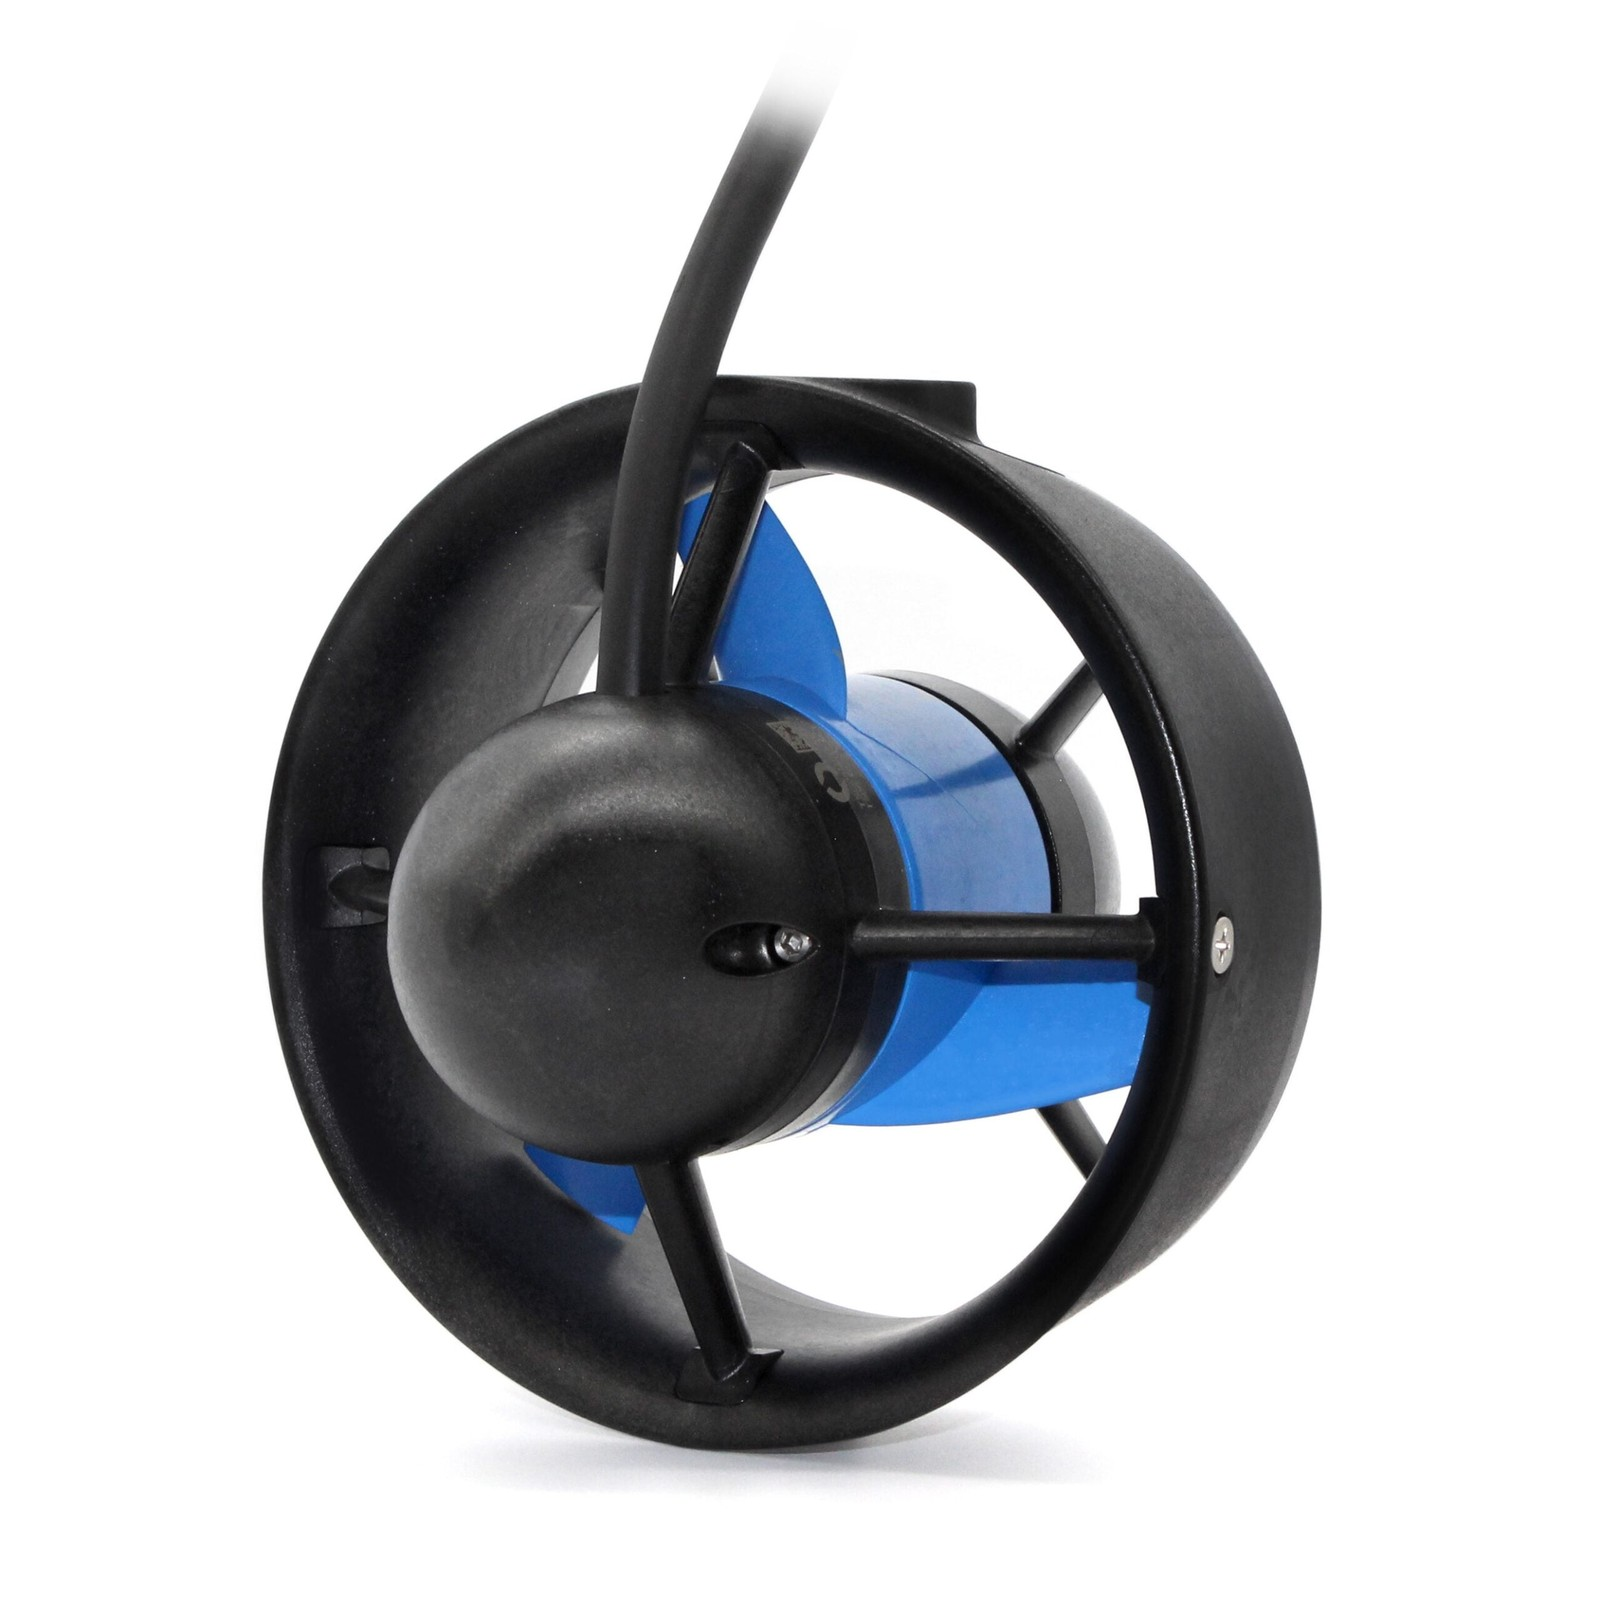
\includegraphics[height=2.3cm, keepaspectratio]{t500_thruster.jpg}\\
        \vspace{0.2em}
        \tech{T500 Thruster}\\
        \footnotesize\textbf{Haute Poussée ($3\times$ T200)}
      \end{center}
      \scriptsize
      \begin{itemize}
        \item Poussée : jusqu'à \succw{$\mathbf{16.1\,\text{kgf}}$} !
        \item Tension nominale : \textbf{$24\,\text{V}$}.
        \item Rendement accru.
        \item Pour gros AUVs, remorquage d'antennes et ASVs rapides.
      \end{itemize}
    \end{column}

    \begin{column}{0.32\textwidth}
      \begin{center}
        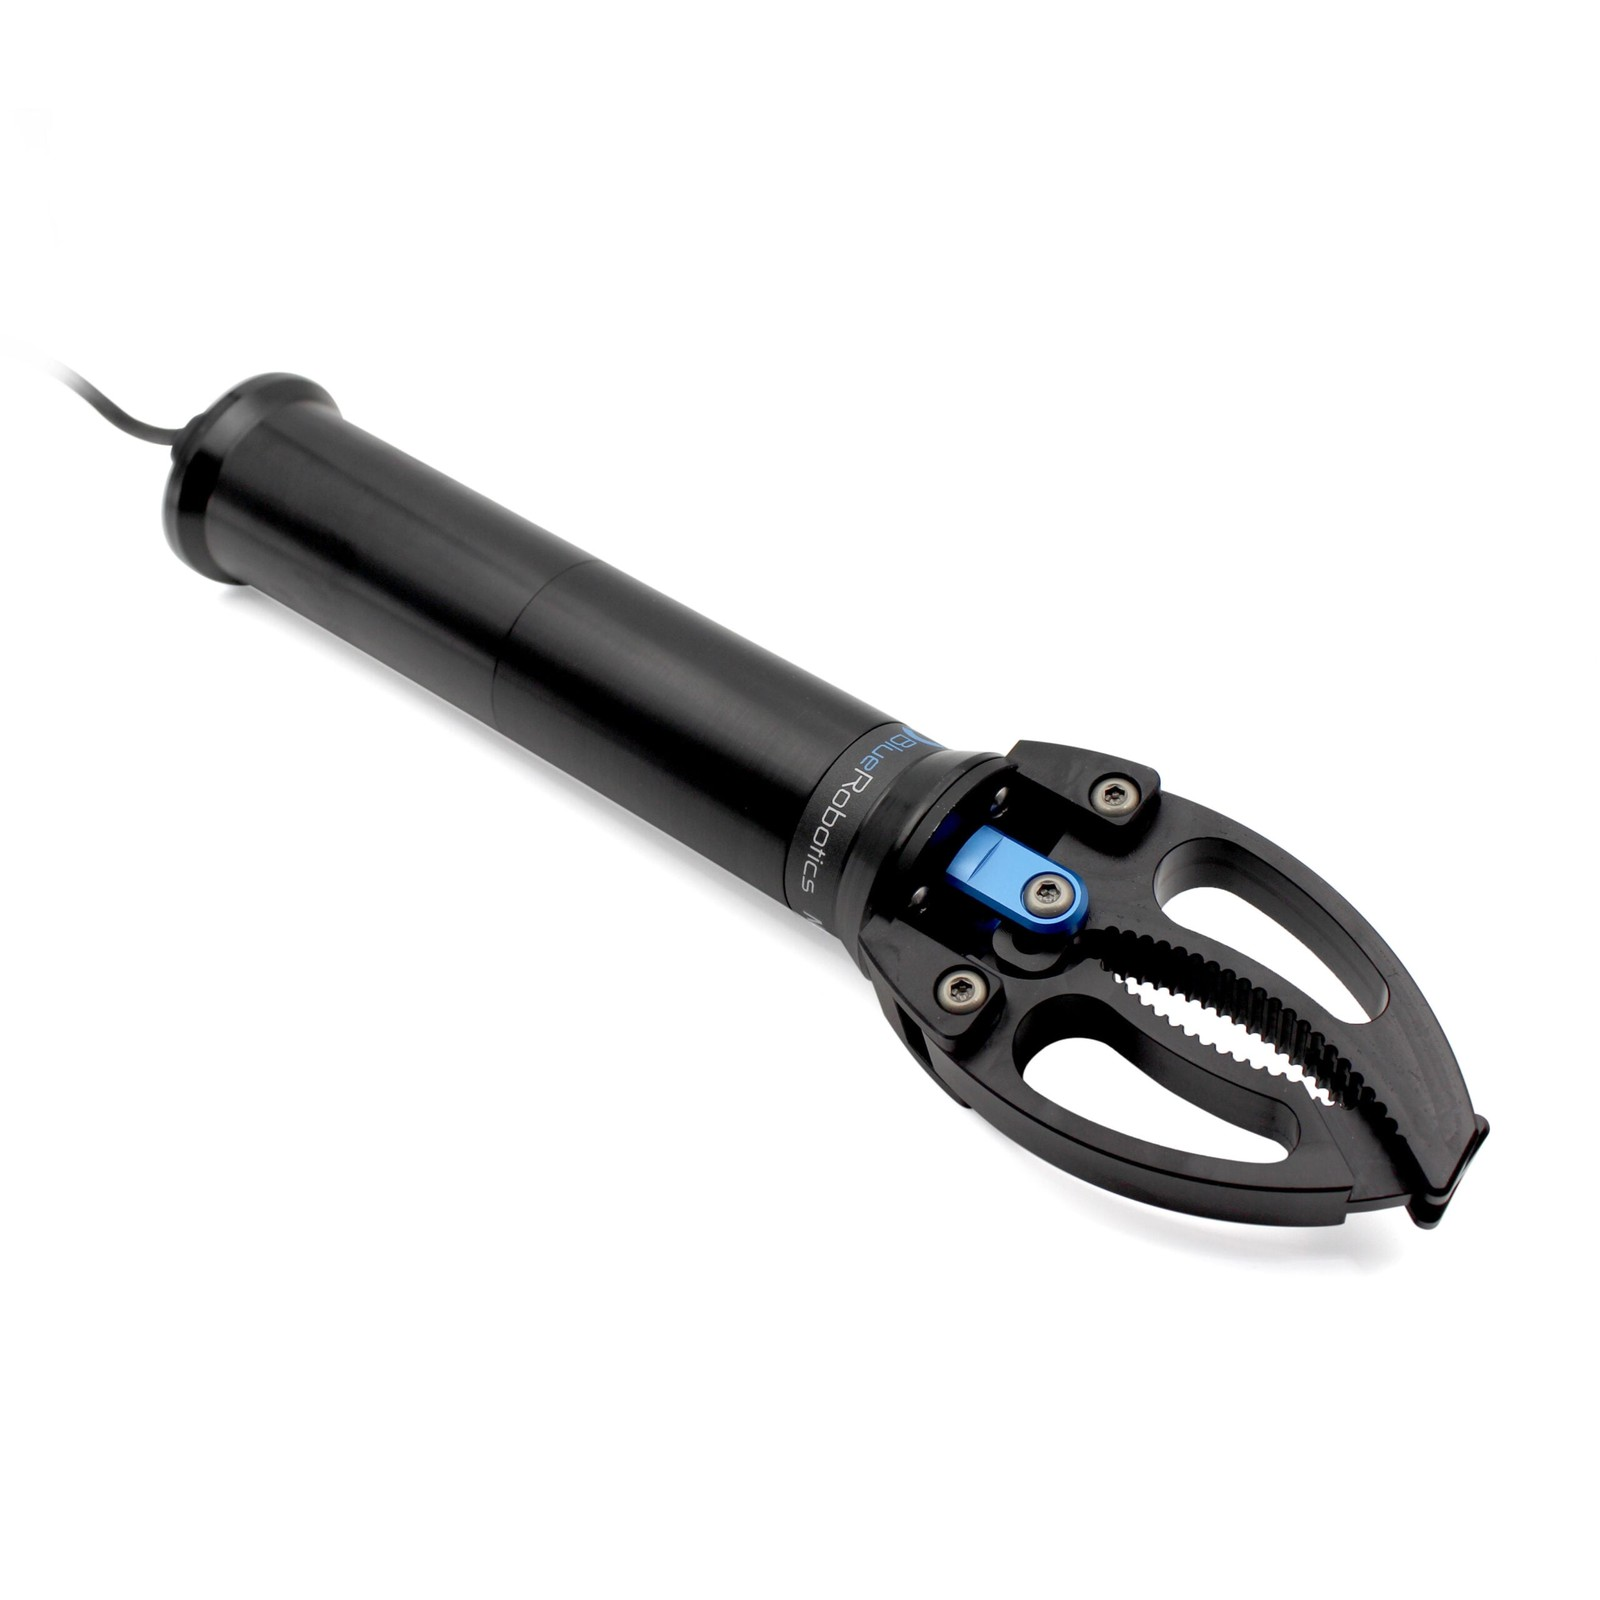
\includegraphics[height=2.3cm, keepaspectratio]{newton_gripper.jpg}\\
        \vspace{0.2em}
        \tech{Pince Newton \& Servos}\\
        \footnotesize\textbf{Actionneur Submersible 300m}
      \end{center}
      \scriptsize
      \begin{itemize}
        \item Commande servo PWM standard ($1.1\text{--}1.9\,\text{ms}$).
        \item Motoréducteur étanche + vis sans fin.
        \item Force de serrage : \textbf{$97\,\text{N}$}.
        \item Prélèvements d'échantillons et largage d'instruments.
      \end{itemize}
    \end{column}
  \end{columns}
\end{frame}

\begin{frame}{1.4 Les Calculateurs : Du Pixhawk à la Carte Navigator}
  \begin{columns}[T]
    \begin{column}{0.42\textwidth}
      \begin{center}
        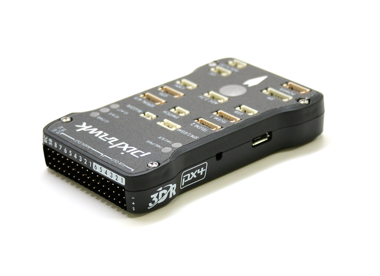
\includegraphics[height=2.2cm, keepaspectratio]{pixhawk_autopilot.png}\\
        \vspace{0.2em}
      \end{center}
      \scriptsize
      \begin{block}{\tech{L'Approche Historique : Pixhawk}}
        \begin{itemize}
          \item Autopilote standard hérité du drone aérien.
          \item Connecté au Raspberry Pi par câble USB/série externe.
          \item Vulnérabilité des connecteurs micro-USB dans les petits caissons étanches.
        \end{itemize}
      \end{block}
    \end{column}

    \begin{column}{0.56\textwidth}
      \begin{center}
        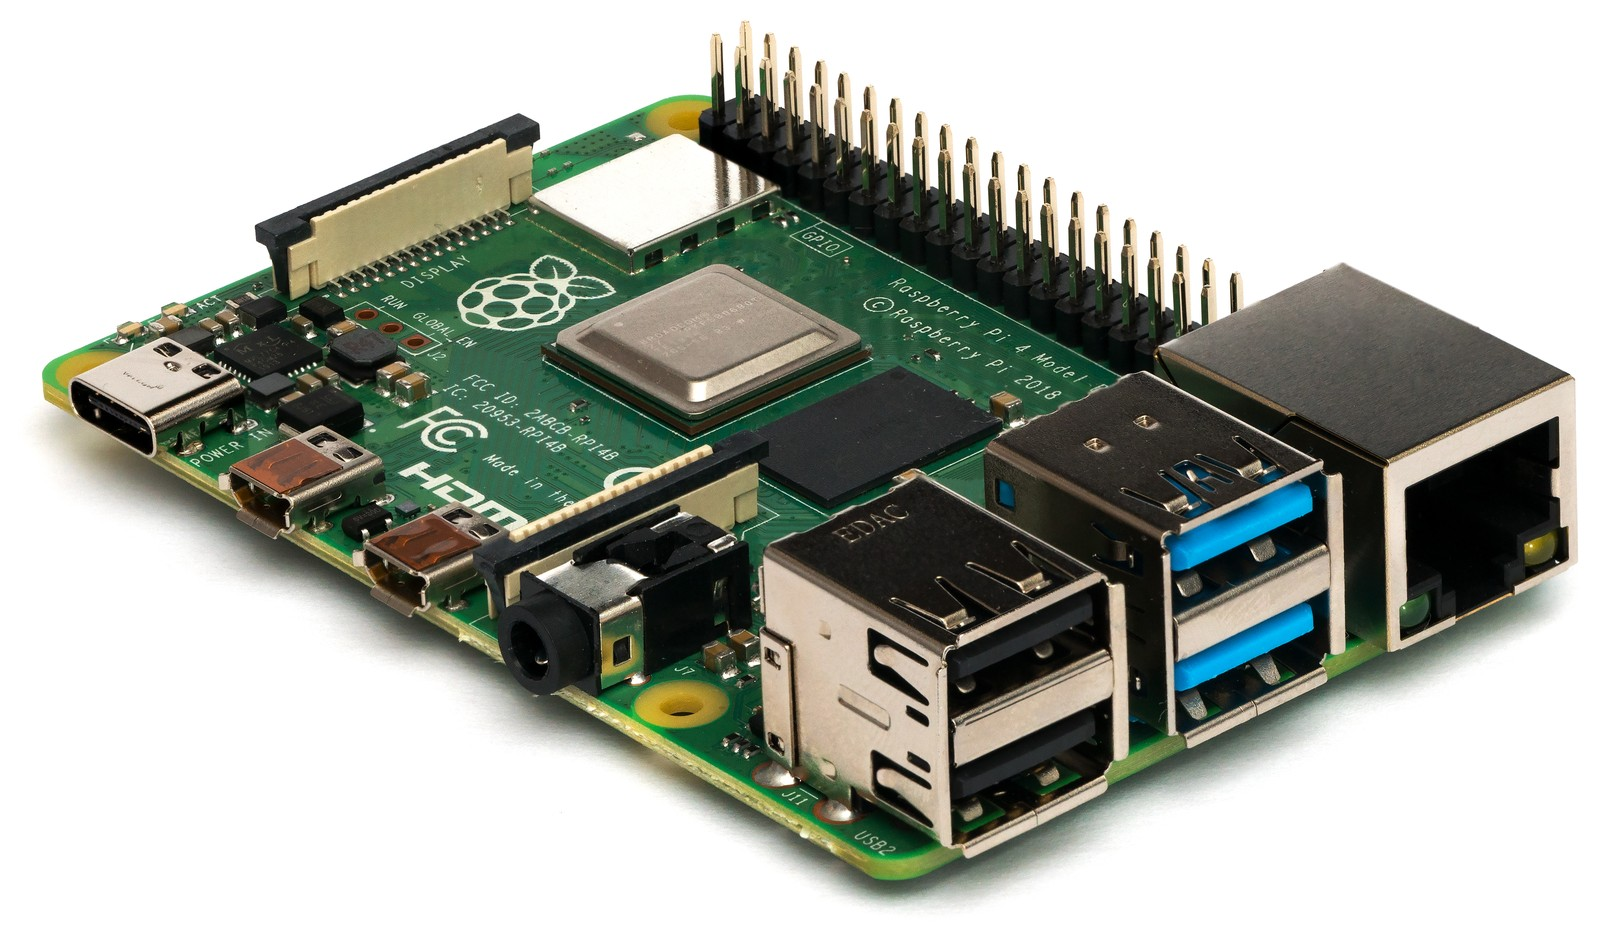
\includegraphics[height=2.0cm, keepaspectratio]{raspberry_pi_4.jpg}
        \hspace{0.3cm}
        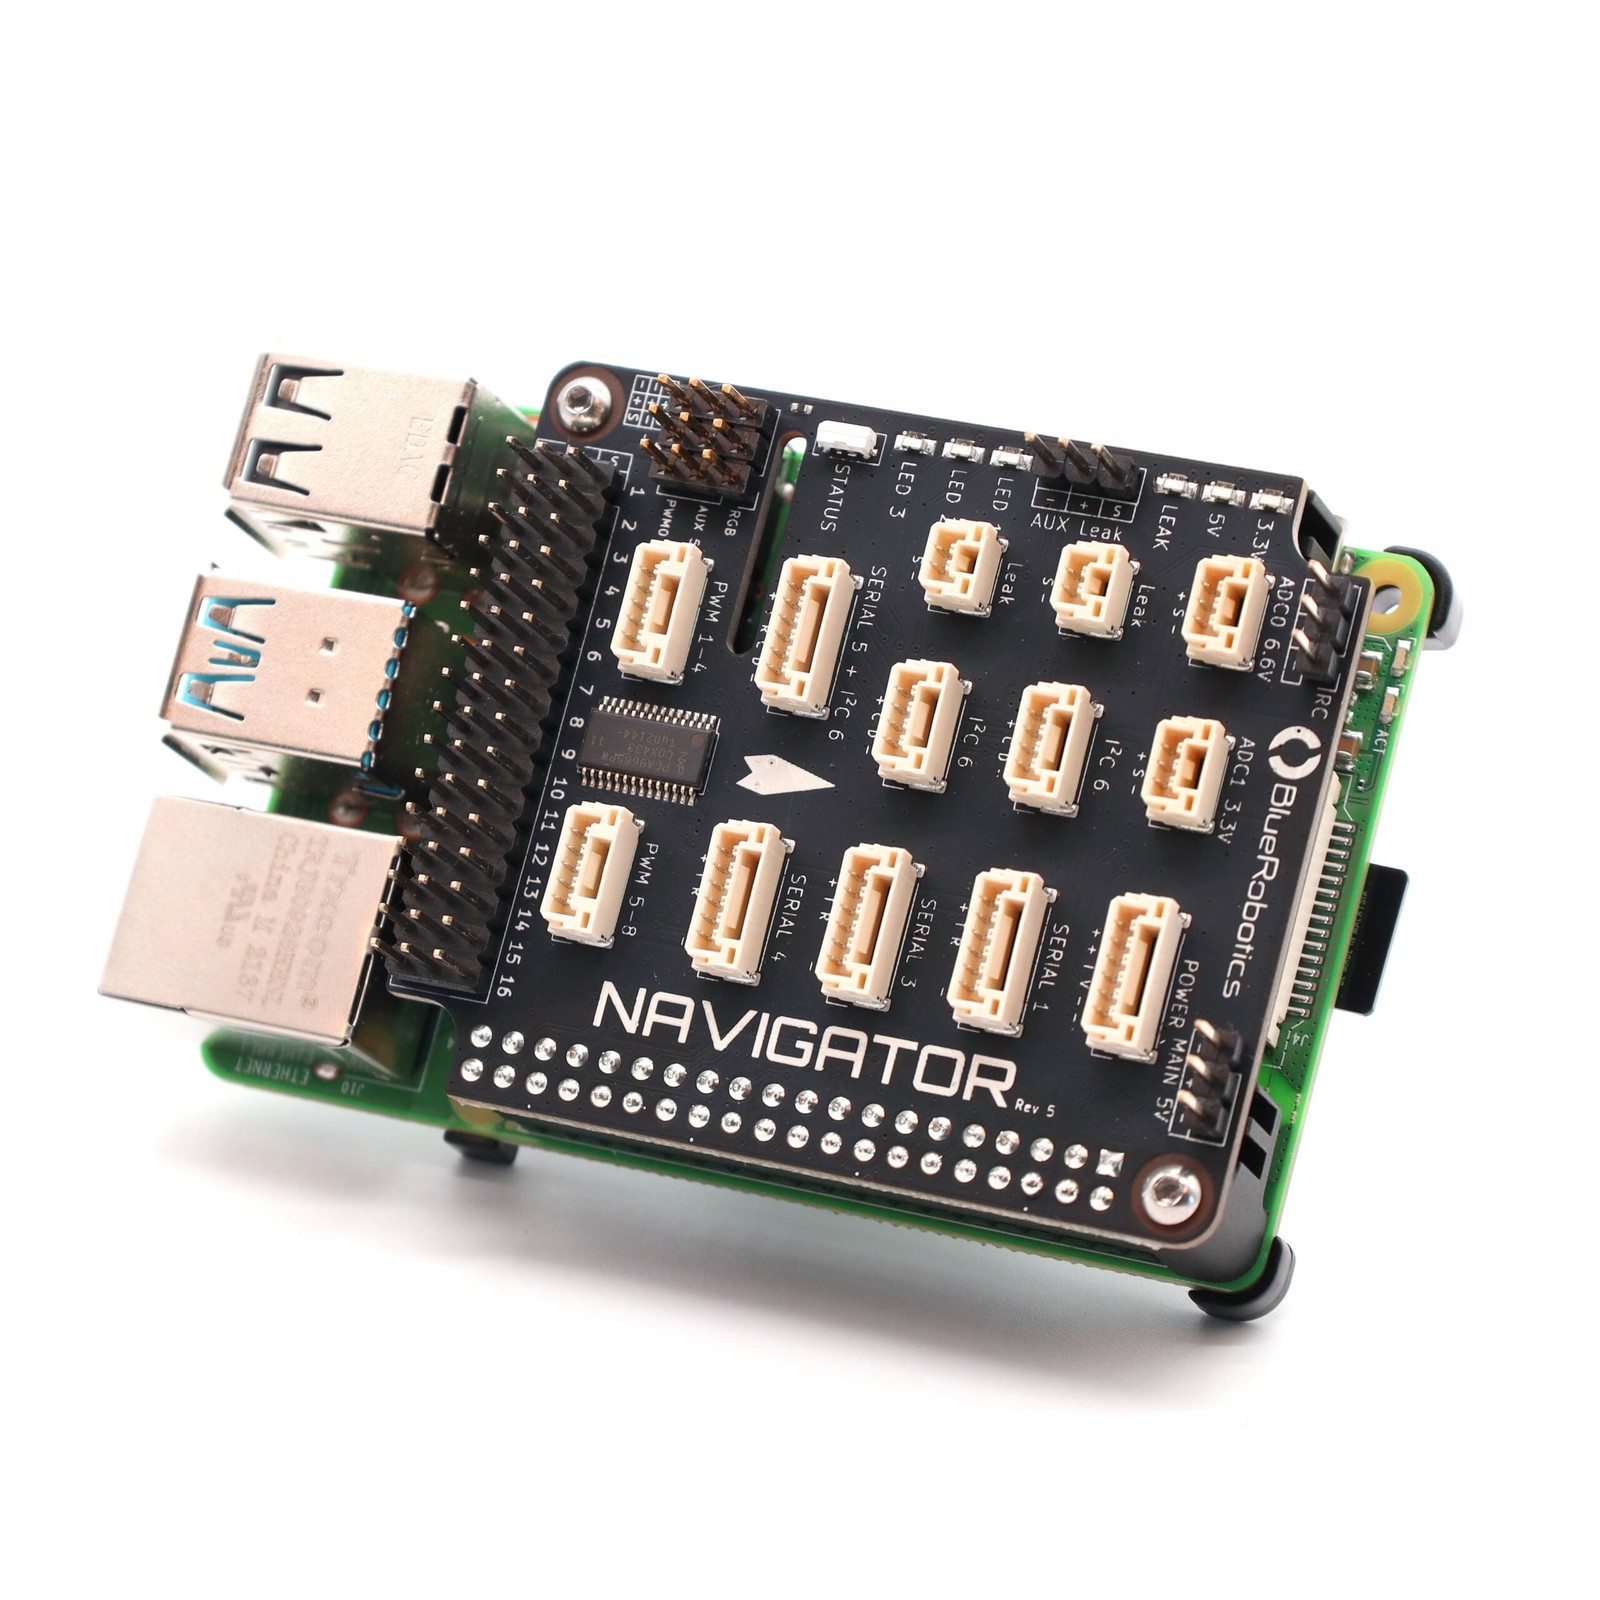
\includegraphics[height=2.0cm, keepaspectratio]{navigator_board.jpg}\\
        \vspace{0.2em}
      \end{center}
      \scriptsize
      \begin{exampleblock}{Le Tandem Moderne : Raspberry Pi 4 + Navigator}
        \begin{itemize}
          \item \textbf{HAT dédié} s'enfichant directement sur le GPIO du \textbf{Raspberry Pi 4 / 5}.
          \item \textbf{Capteurs intégrés} : double IMU redondante (ICM-20602 + ICM-20948), magnétomètre MMC5983MA, pression interne.
          \item \textbf{Connectique native} : 16 sorties PWM, bus I2C, ADC, ports séries (JST-GH).
          \item Une seule alimentation, zéro câble USB interne !
        \end{itemize}
      \end{exampleblock}
    \end{column}
  \end{columns}
\end{frame}

\begin{frame}{1.5 Mesure de Profondeur : Les Capteurs Bar30 et Bar02}
  \begin{center}
    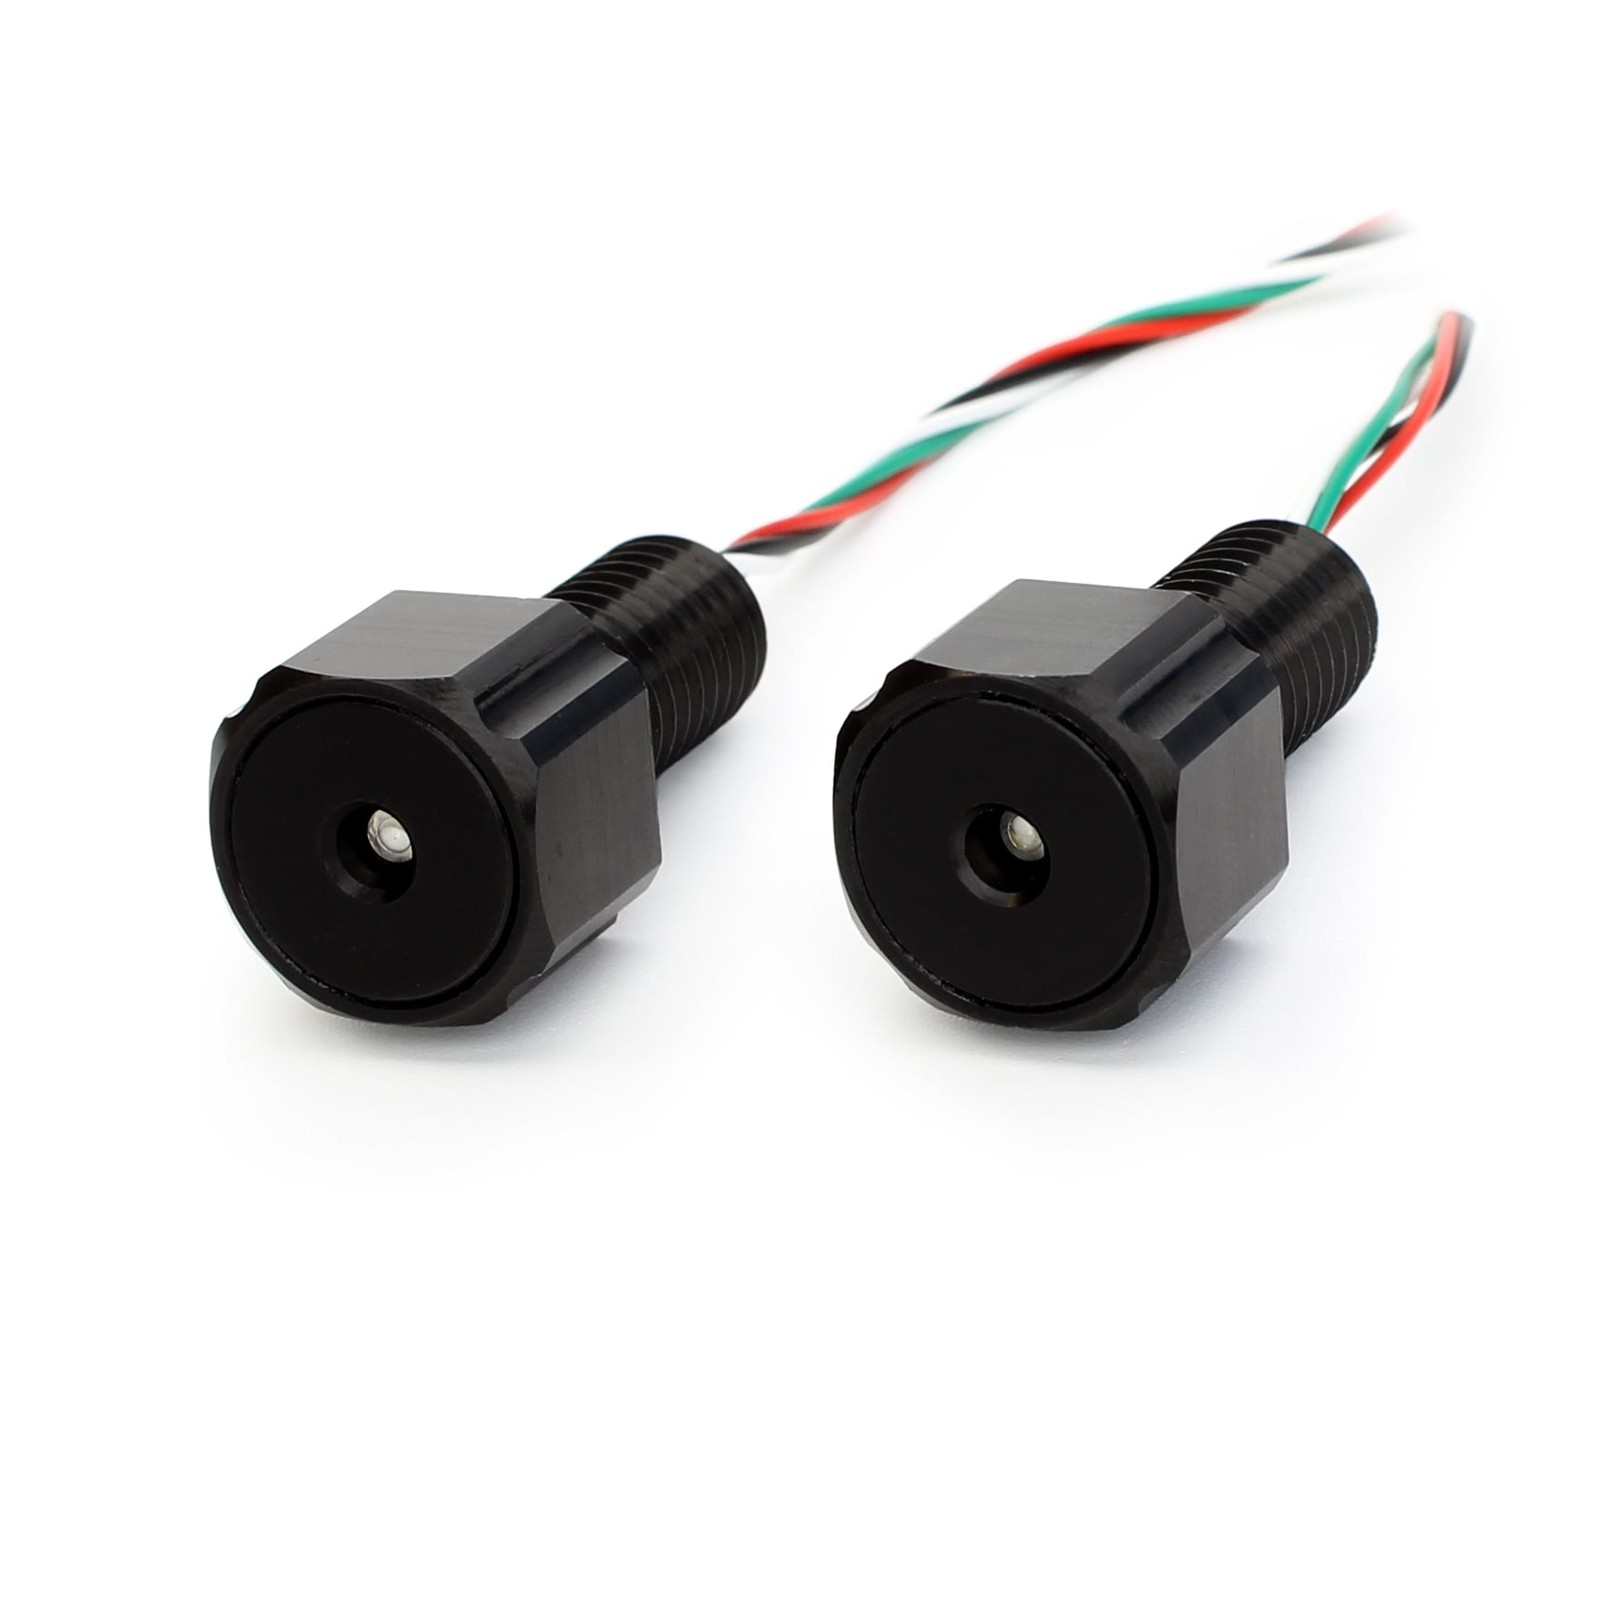
\includegraphics[trim=30 130 30 50, clip, height=2.3cm, keepaspectratio]{bar30_sensor.jpg}\\[0.2em]
    \footnotesize\tech{Boîtier M10 Étanche Commun (Bar30 \& Bar02)}\\
    \scriptsize\textcolor{DarkSlate!70}{Corps aluminium anodisé M10 étanche, joint torique, interface numérique bus I\textsuperscript{2}C (3.3\,V, adresse \code{0x76}).}
  \end{center}
  \vspace{-0.3em}
  \begin{columns}[T]
    \begin{column}{0.48\textwidth}
      \begin{block}{\tech{Capteur Bar30 (MS5837-30BA)}}
        \scriptsize
        \begin{itemize}
          \item \textbf{Gamme} : $0\text{--}30\,\text{bar}$ ($0\text{--}300\,\text{m}$ de profondeur).
          \item \textbf{Résolution} : \succw{$\mathbf{0.2\,\text{mm}}$ d'eau} ($0.16\,\text{mbar}$).
          \item \textbf{Usage cible} : ROVs \& AUVs côtiers (BlueROV2).
          \item \textbf{Contrôle} : Asservissement vertical fin (\textit{Depth Hold}).
          \item \textbf{Tarif indicatif} : \tech{$\approx 80\,\$$} (missions intermittentes).
        \end{itemize}
      \end{block}
    \end{column}
    \begin{column}{0.48\textwidth}
      \begin{block}{\tech{Capteur Bar02 (MS5837-02BA)}}
        \scriptsize
        \begin{itemize}
          \item \textbf{Gamme} : $0\text{--}2\,\text{bar}$ ($0\text{--}10\,\text{m}$ de profondeur / surface).
          \item \textbf{Résolution} : \succw{$<\mathbf{0.05\,\text{mm}}$ d'eau} (ultra-fine).
          \item \textbf{Technologie} : Silicium piézorésistif sous gel.
          \item \textbf{Usage cible} : Lacs, marégraphes, houle sur ASV.
          \item \textbf{Entretien} : Rinçage eau douce post-mission obligatoire.
        \end{itemize}
      \end{block}
    \end{column}
  \end{columns}
\end{frame}

\begin{frame}{1.5b Immersion Continue : Capteurs Haute Résistance BarXT}
  \begin{columns}[c]
    \begin{column}{0.44\textwidth}
      \begin{center}
        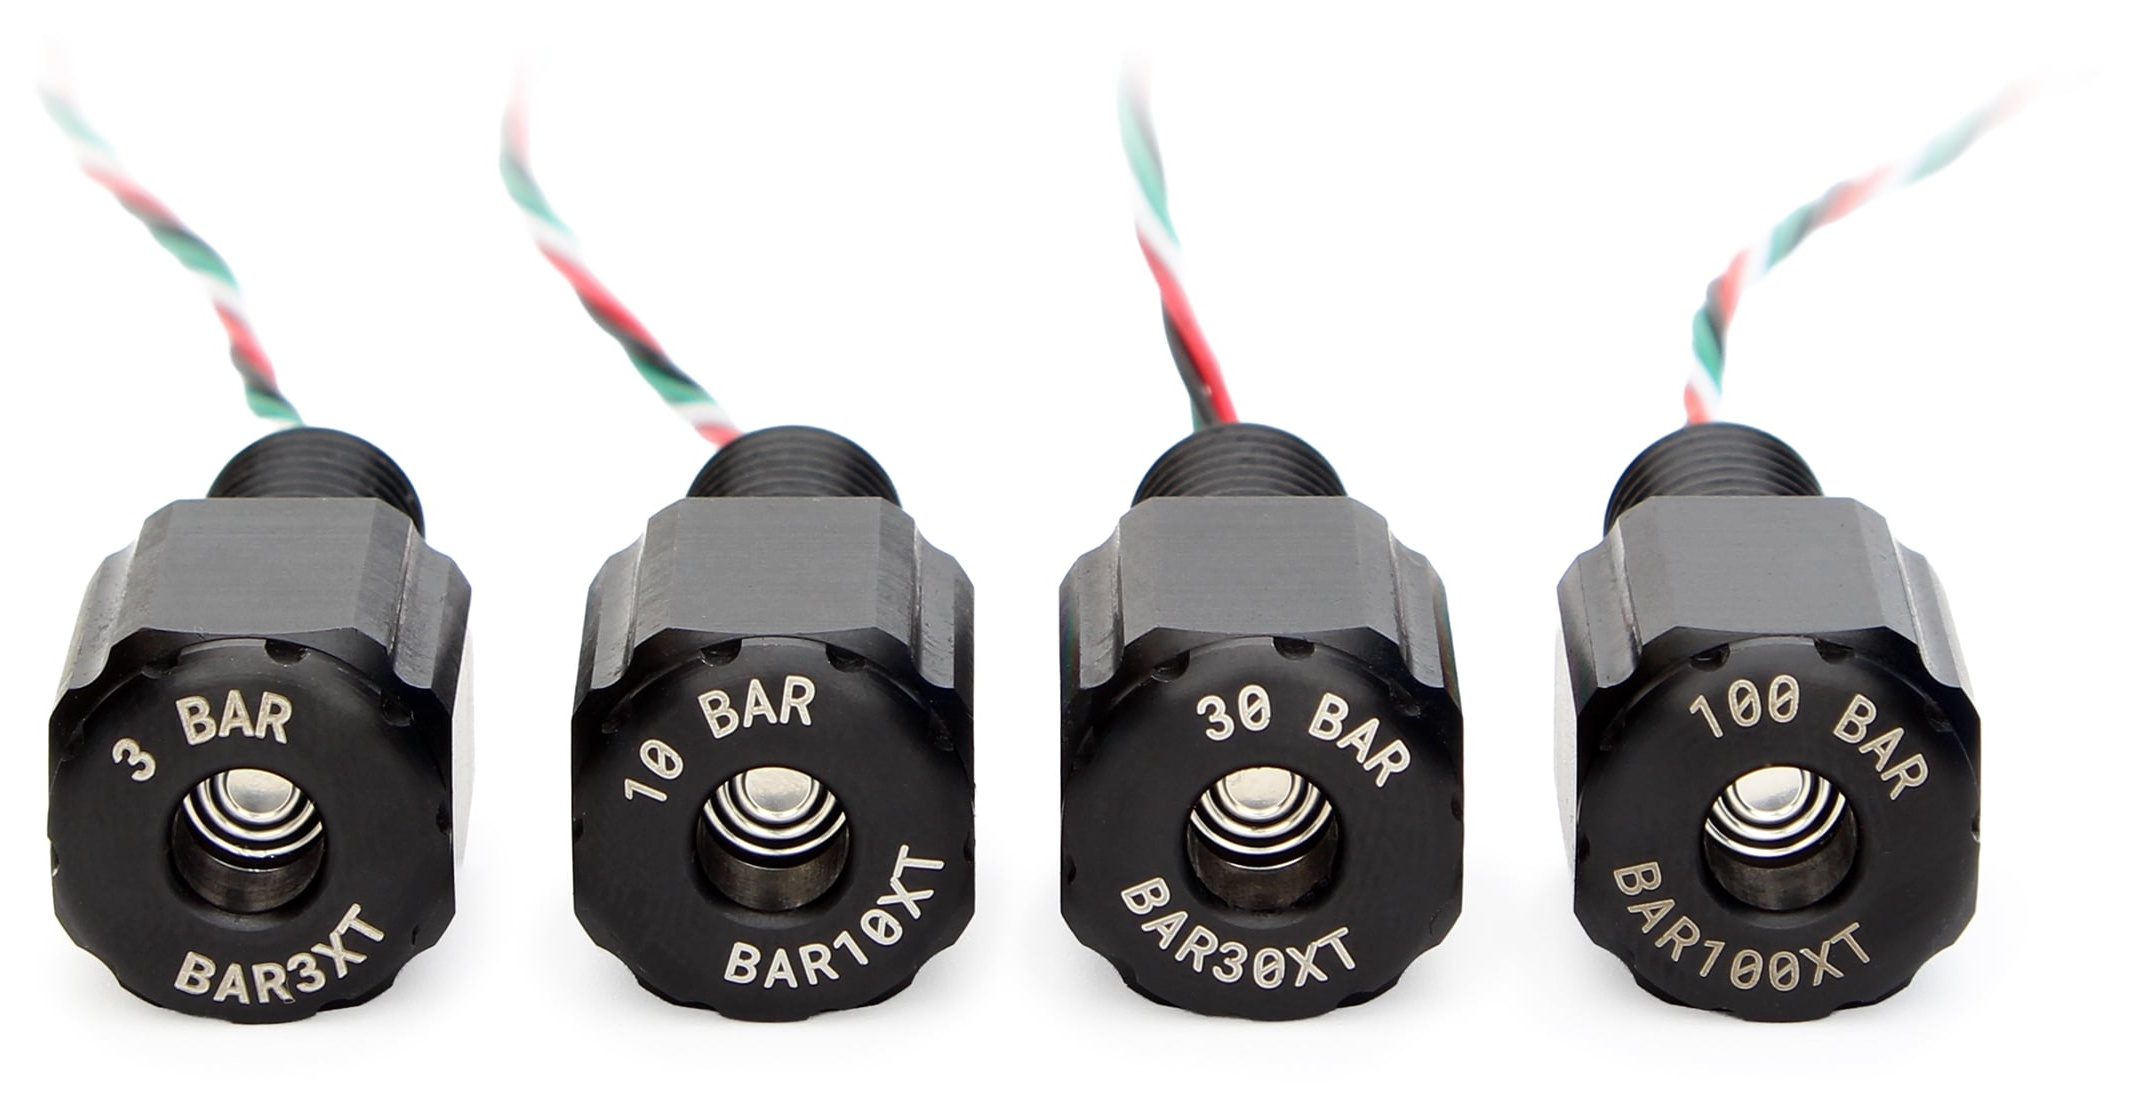
\includegraphics[height=1.65cm, keepaspectratio]{barxt_sensor_clean.jpg}\\[0.2em]
        \footnotesize\tech{Série Blue Robotics BarXT (\textit{Extended Submersion})}\\[0.1em]
        \scriptsize\textcolor{DarkSlate!70}{Corps Inox 316L oxyde noir, capteur soudé Keller 4LD, bus I\textsuperscript{2}C (\code{0x40}).}
      \end{center}
    \end{column}
    \begin{column}{0.54\textwidth}
      \begin{alertblock}{La Limite des Capteurs Standard ($\approx 80\,\$$)}
        \scriptsize
        \begin{itemize}
          \item \textbf{Gel silicone en contact} : colmatage par \textit{biofouling} et hydrolyse en immersion permanente.
          \item \textbf{Aluminium M10} : sensibilité à la corrosion galvanique.
          \item Rinçage eau douce et séchage obligatoires post-mission.
        \end{itemize}
      \end{alertblock}
    \end{column}
  \end{columns}

  \vspace{0.15em}

  \begin{columns}[T]
    \begin{column}{0.48\textwidth}
      \begin{block}{\tech{Atouts Technologiques BarXT}}
        \scriptsize
        \begin{itemize}
          \item \textbf{Immersion indéfinie} : conçu pour stations fond de mer, bouées \& mouillages scientifiques permanents.
          \item \textbf{Cellule Keller 4LD scellée} : membrane inox soudée, huile isolante, zéro gel exposé.
          \item \textbf{Protection mécanique} : capot frontal ajouré.
          \item \textbf{Gamme étendue} : de $3\,\text{bar}$ jusqu'à \succw{$100\,\text{bar}$ ($1000\,\text{m}$)}.
        \end{itemize}
      \end{block}
    \end{column}

    \begin{column}{0.48\textwidth}
      \begin{exampleblock}{Arbitrage Opérationnel : $80\,\$$ vs $380\,\$$}
        \scriptsize
        \begin{itemize}
          \item \textbf{Bar30 / Bar02 ($\approx 80\,\$$)} : parfait pour ROVs d'inspection, drones de surface, plongées courtes.
          \item \textbf{Série BarXT ($\approx 380\,\$$)} : facteur \alertw{$\approx 4.7\times$} de surcoût à l'achat.
          \item \textbf{Rentabilité terrain} : le delta de $\sim 300\,\$$ est négligeable face au coût d'une campagne navale pour remplacer un capteur dérivé ou colmaté.
        \end{itemize}
      \end{exampleblock}
    \end{column}
  \end{columns}
\end{frame}

\begin{frame}{1.6 Les Autopilotes Open-Source : ArduSub vs ArduRover vs PX4}
  \begin{table}[h]
    \centering
    \small
    \begin{tabularx}{\textwidth}{l p{3.2cm} p{3.2cm} X}
      \toprule
      \textbf{Autopilote} & \textbf{Vecteur Cible} & \textbf{Modes Clés} & \textbf{Intérêt Scientifique} \\
      \midrule
      \tech{ArduSub} & ROVs \& AUVs subaquatiques & Stabilize, \textbf{Depth Hold}, Auto, PosHold (DVL) & Asservissement vertical fin via Bar30, gestion de 6 à 8 thrusters vectoriels. \\
      \rowcolor{OceanGray}
      \tech{ArduRover} & ASV / Drones de surface (\textbf{BlueBoat}) & Manual, Acro, \textbf{Auto Survey}, RTL & Navigation différentielle (*skid-steering*), quadrillage bathymétrique par GPS. \\
      \tech{PX4} & Aérien / sous-marin expérimental & Offboard, Position, Mission & Architecture orientée micro-services, pont micro-ROS / uORB natif. \\
      \bottomrule
    \end{tabularx}
  \end{table}

  \begin{block}{Le Protocole MAVLink : La Passerelle Universelle}
    Toutes les données de vol (attitude, tension batterie, profondeur Bar30, alertes fuite) sont encapsulées dans des paquets \textbf{MAVLink} légers, standardisés et lisibles par n'importe quel langage (Python via \code{pymavlink}, C++, ROS via \code{mavros}).
  \end{block}
\end{frame}

\begin{frame}{1.7 Cadre Réglementaire Français : Le Statut du Drone Maritime}
  \begin{columns}[T]
    \begin{column}{0.49\textwidth}
      \begin{block}{\tech{Textes Fondateurs en Droit Français}}
        \scriptsize
        \begin{itemize}
          \item \href{https://www.legifrance.gouv.fr/jorf/id/JORFTEXT000044202140}{\underline{\textbf{Ordonnance n° 2021-1330}}} (13 oct. 2021) : statut des navires autonomes et drones.
          \item \href{https://www.legifrance.gouv.fr/jorf/id/JORFTEXT000049583905}{\underline{\alertw{Décret n° 2024-461}}} (22 mai 2024) : exploitation, sécurité et formation.
          \item \textbf{Code des transports} :
            \begin{itemize}\scriptsize
              \item \href{https://www.legifrance.gouv.fr/codes/article_lc/LEGIARTI000049585210}{\underline{\tech{Art. R. 5000-1}}} : Définition légale stricte.
              \item \href{https://www.legifrance.gouv.fr/codes/article_lc/LEGIARTI000049585847}{\underline{\tech{Art. R. 5241-2}}} : Navigation subaquatique.
              \item \href{https://www.legifrance.gouv.fr/codes/article_lc/LEGIARTI000049586745}{\underline{\tech{Art. R. 5271-1}}} : Titres et qualifications.
            \end{itemize}
        \end{itemize}
      \end{block}

      \vspace{-0.3em}
      \begin{block}{\succw{Obligation du Brevet Capitaine 200}}
        \scriptsize
        La recherche en mer relève du \textbf{secteur professionnel}. La responsabilité légale nautique et le respect du RIPAM (COLREG 72) imposent la présence ou supervision d'un marin breveté \alertw{Capitaine 200} (Marine Marchande) sur le navire support ou au centre de télé-opération (COD).
      \end{block}
    \end{column}

    \begin{column}{0.49\textwidth}
      \begin{alertblock}{Critères Cumulatifs Drone Maritime (\code{Art. R. 5000-1})}
        \scriptsize
        Engin flottant de surface ou sous-marin opéré à distance / autonome sans personne à bord :
        \begin{itemize}\scriptsize
          \item \textbf{Longueur hors-tout} : $1\,\text{m} < L_{\text{HT}} < 16\,\text{m}$.
          \item \textbf{Vitesse maximale} : $\le 20\,\text{n\oe uds}$ ($\approx 37\,\text{km/h}$).
          \item \textbf{Énergie cinétique} : $< 300\,\text{kJ}$ ($\frac{1}{2} M V_{\max}^2$).
          \item \textbf{Jauge brute} : $< 100$.
        \end{itemize}
      \end{alertblock}

      \vspace{-0.3em}
      \begin{exampleblock}{Exclusions Expresses (\code{Art. R. 5000-1})}
        \scriptsize
        \begin{itemize}\scriptsize
          \item \textbf{Micro-engins} : longueur $\le 1.00\,\text{m}$.
          \item \textbf{Bande des 300 mètres} : engins radiocommandés sous police du maire.
          \item \textbf{Objets non man{\oe}uvrants} : bouées et gliders dérivants.
        \end{itemize}
      \end{exampleblock}
    \end{column}
  \end{columns}
\end{frame}

\begin{frame}{1.7b Déploiement Scientifique : Astuces Légales \& Contournements}
  \begin{columns}[T]
    \begin{column}{0.49\textwidth}
      \begin{block}{\tech{3 Leviers pour Alléger les Contraintes}}
        \scriptsize
        \begin{itemize}
          \item \textbf{1. Le ROV filaire (BlueROV2)} : relié en permanence par ombilical. Qualifié d'\textbf{équipement captif immergé} sous la garde du bateau/quai $\rightarrow$ \succw{zéro qualification drone requise} !
          \item \textbf{2. Le seuil des $\le 1\,\text{m}$ (Micro-AUV)} : l'\href{https://www.legifrance.gouv.fr/codes/article_lc/LEGIARTI000049585210}{\underline{\code{Art. R. 5000-1}}} impose $L > 1\,\text{m}$. Un engin $\le 1\,\text{m}$ \succw{échappe à la qualification de drone maritime} (modélisme naval / outil scientifique léger).
          \item \textbf{3. Bande des 300 m \& Eaux intérieures} : à vue à $<300\,\text{m}$ du rivage (police du maire, autorisations simples) ou en lacs/fleuves (régime VNF / DDTM).
        \end{itemize}
      \end{block}
    \end{column}

    \begin{column}{0.49\textwidth}
      \begin{alertblock}{4. Navire Support avec Capitaine 200}
        \scriptsize
        En mer ouverte avec un ASV $>1\,\text{m}$ (BlueBoat) ou AUV :
        \begin{itemize}\scriptsize
          \item Naviguer avec un semi-rigide d'escorte à vue immédiate.
          \item \alertw{Embarquer un marin Capitaine 200} (agent breveté du labo, skipper station marine CNRS ou prestataire).
          \item Le Capitaine 200 assure la veille optique 360°, la liaison VHF 16 avec le CROSS et la responsabilité RIPAM.
        \end{itemize}
      \end{alertblock}

      \vspace{-0.3em}
      \begin{exampleblock}{5. Déclaration Prémar \& AVURNAV}
        \scriptsize
        Déclaration d'expérimentation DML / Préfecture Maritime : publication d'un \textbf{AVURNAV} temporaire réservant la zone aux navigateurs tiers.
      \end{exampleblock}
    \end{column}
  \end{columns}
\end{frame}

\begin{frame}{1.7c Sécuriser sa Zone : La Plateforme PING (Shom / DGAMPA)}
  \begin{columns}[T]
    \begin{column}{0.52\textwidth}
      \begin{block}{\tech{Qu'est-ce que la Plateforme PING ?}}
        \scriptsize
        \begin{itemize}
          \item \textbf{P}lateforme d'\textbf{I}nformation \textbf{N}autique \textbf{G}éoréférencée : portail officiel développé conjointement par le \textbf{Shom} et la \textbf{DGAMPA}.
          \item Accessible en ligne : \href{https://portail.ping-info-nautique.fr/}{\underline{\tech{portail.ping-info-nautique.fr}}}
          \item Également intégrée dans l'application mobile \textbf{Nav\&Co} (Shom / Office Français de la Biodiversité).
          \item Outil de référence pour la sécurité maritime en France (Manche, Atlantique, Méditerranée, Outre-mer).
        \end{itemize}
      \end{block}

      \begin{alertblock}{Le Réflexe Avant Toute Mise à l'Eau}
        \scriptsize
        Consulter PING le matin même de la manip : un polygone de tir temporaire non anticipé peut entraîner l'interception de votre drone par les vedettes de la Marine ou des Affaires Maritimes.
      \end{alertblock}
    \end{column}

    \begin{column}{0.46\textwidth}
      \begin{exampleblock}{Informations Clés Diffusées sur PING}
        \scriptsize
        \begin{itemize}
          \item \textbf{Avis aux Navigateurs} : cartographie spatialisée des \alertw{AVURNAV} (urgents) et \textbf{AVINAV} (locaux).
          \item \textbf{Zones d'Exclusion Militaires} : polygones de tir réel, essais sous-marins et torpillages.
          \item \textbf{Couloirs de Navigation} : Dispositifs de Séparation de Trafic (DST) et chenaux d'accès aux ports.
          \item \textbf{Restrictions Environnementales} : cantonnements, réserves naturelles, arrêtés préfectoraux de mouillage (ex: Posidonie).
          \item \textbf{Infrastructures Sous-Marines} : câbles télécoms, émissaires et épaves.
        \end{itemize}
      \end{exampleblock}
    \end{column}
  \end{columns}
\end{frame}

\begin{frame}{Synthèse du Module 1 : Briques Matérielles \& Cadre Opérationnel}
  \begin{exampleblock}{La recette gagnante pour un drone scientifique opérationnel}
    \begin{enumerate}
      \item \textbf{Base mécanique éprouvée} : coque ouverte modulaire (BlueROV2 ou BlueBoat).
      \item \textbf{Motorisation robuste} : propulseurs T200 étanches par conception et ESCs réversibles.
      \item \textbf{C{\oe}ur numérique intégré} : couple Raspberry Pi 4 + Navigator (Linux + temps réel).
      \item \textbf{Capteur environnemental clé} : capteur de pression Bar30 (résolution millimétrique).
      \item \textbf{Logiciel pérenne} : ArduSub ou ArduRover pour l'asservissement fiable en boucle fermée.
      \item \textbf{Cadrage réglementaire} : consultation de PING et choix du cadre (ROV captif, $\le 1\,\text{m}$ ou Capitaine 200).
    \end{enumerate}
  \end{exampleblock}

  \begin{alertblock}{La prochaine étape : L'étanchéité et le passage de câbles}
    Comment assembler ces composants pour qu'ils résistent à la pression sans couler ? Rendez-vous au Module 2 avec les caissons 4 pouces, les pénétrateurs WetLink, les connecteurs étanches Cobalt/SubConn et le BlueBoat !
  \end{alertblock}
\end{frame}
